\documentclass[12pt,letterpaper ,oneside , openright]{book}
\usepackage{thesis}
%para desarrollo
	%\usepackage{showframe}
	%\includeonly{calculatingProperties_chapter,calculatingProperties/parameters,calculatingProperties/enthalpy}
%--

\begin{document}
	\begin{titlepage}
	\begin{minipage}[c][9in][s]{1in}
	\centering
	\includegraphics[width=1in]{Escudo-UNAM}\\[10pt]
	\hskip 2pt\vrule width 2pt height 6.7in
	\hskip 1mm\vrule width 1pt height 6.7in\\[10pt]
	\includegraphics[width=1in]{images/FQ.jpg}
	\end{minipage}\hskip 10pt
	\begin{minipage}[c][\textheight][s]{5.125in}
	\centering
	{\textsc{ \large{Universidad Nacional Autónoma De México}}}
	\vspace{3mm}\hrule height2pt
	\vspace{1mm}\hrule height1pt
	\vspace{3mm}
	\textsc{Facultad De Química}\\[3cm]
	\textsc{\Large Desarrollo de una librería en java para el cálculo de propiedades de sustancias con ecuaciones de estado cúbicas}\\[3cm]
	\makebox[8cm][s]{\Huge T E S I S}\\[8pt]
	\textsc{ que para obtener el título de }\\[3pt]
	\textsc{ Ingeniero Químico}\\[1cm]
	\textsc{ presenta: }\\[0.3cm]
	\textsc{ Hugo Redon Rivera }\\[0.5cm]
	\vfill
	{\scshape {México, D.F.} \hfill{2014} }	
	\end{minipage}
\end{titlepage}
\newpage
\begin{minipage}[c][\textheight][s]{5.125in}
JURADO ASIGNADO:\\[0.5cm]

PRESIDENTE:		Profesor: Enrique Rodolfo Bazúa Rueda\\
VOCAL: 		Profesor:Jose Fernando Barragán Aroche\\
SECRETARIO:		Profesor: Ernesto Jose Calderón Castillo\\
1er.  SUPLENTE: 	Profesor: Emma Gonzalez Chimeo\\
2° SUPLENTE:		Profesor: Milton Thadeu García Medeiros de Oliveira\\[0.5cm]

\begin{center}
	SITIO DONDE SE DESARROLLÓ EL TEMA:\\
	\textsc{Facultad de Química}\\[3cm]


	\rule{6cm}{1pt}\\
	\textsc{asesor del tema: Dr. Enrique Rodolfo Bazúa Rueda.} \\[3cm]


	\rule{6cm}{1pt}\\
	\textsc{SUSTENTANTE:Hugo Redon Rivera.} 
\end{center}
\end{minipage}
%Portada -Hecho
	\tableofcontents	
	\chapter{Objetivos}

\begin{itemize}
	\item Desarrollar una librería escrita en el lenguaje de java para el cálculo de propiedades de sustancias con ecuaciones de estado cúbicas.
	\item Desarrollar un programa que exponga las funciones de la librería.
	\item Proponer un medio de difusión de la librería, que sea capaz de involucrar a cualquier persona interesada en modificar y extender la librería.
\end{itemize}
%Objetivos -Hecho
	\chapter{Herramientas}\label{chap:tools}

	Las herramientas que se describen en este capítulo en conjunto con la librería \textbf{Materia} forman la plataforma de desarrollo propuesta en esta tesis. Estas herramientas dan la versatilidad necesaria para el desarrollo de futuras aplicaciónes de modelado y simulación. 

	Las herramientas resuelven las siguientes necesidades:

\begin{itemize}
	\item Java nos permite el desarrollo de los métodos computacionales de una forma sencilla y segura.
	\item JUnit asegura el funcionamiento de la librería sin importar los cambios que sean introducidos al código.
	\item Git permite administrar los cambios entre versiones de una forma segura.
	\item GitHub guarda el código fuente y permite compartir los cambios a través de internet.
	\item Maven permite construir las aplicaciones descargando las proyectos necesarios desde los servidores centrales de Maven.
	\item Netbeans es el ambiente de desarrollo que permite escribir, compilar y ejecutar las aplicaciones escritas.
	\item Licencia `GNU GENERAL PUBLIC LICENSE Version 2' asegura que el código fuente sea libre para todos los usuarios.%usado segun las condiciones deseadas.
	\item Idioma inglés, mantiene una fluidez en la lectura del código fuente.
\end{itemize}

	\section{Java}

		James Gosling \footnote{Considerado creador del lenguaje Java} define a java como: 

		Un lenguaje simple, orientado a objetos, distribuido, interpretado, robusto, de arquitectura neutral, portátil, de alto rendimiento, seguro, multiproceso y dinámico.\cite{java}

		

		\begin{description}
		\item{Simple:} Una de las razones mas importantes por las que se decidió programar la librería en este lenguaje, es que java evita al programador la necesidad de realizar tareas de índole técnico sobre la computadora, como por ejemplo el almacenamiento de los datos en la memoria. Esto permite al programador concentrarse en el area de estudio deseada.

		\item{Orientado a objetos:}
		Sin duda la perspectiva orientada a objetos de java es otro gran atractivo para las ciencias e ingenierías. La división y clasificación de las ramas de estudio permiten concentrarnos en todos y cada uno de los aspectos importantes sobre el tema. De igual manera la division de un programa en objetos nos permite concentrarnos en los aspectos y actividades importantes del programa. Tómese como ejemplo la clasificación de la materia en homogénea y heterogénea, el aspecto importante en esta clasificación es la presencia de uno o más estados de agregación en el sistema, se puede pensar así en un cálculo de equilibrio Líquido-Vapor para un sistema heterogéneo, pero no para un sistema homogéneo.

		\item{Distribuido:}
		Java es una de las principales herramientas para el desarrollo web. La importancia del desarrollo web radica en su capacidad de difusión masiva. La difusión de un servicio o producto es tan importante como su creación. En conjunto con la librería de funciones se ha creado un sitio web donde se exponen algunas de las funciones mas importantes de la librería.

		\item{De arquitectura neutra:}
		Java es multiplataforma, lo cual significa que puede ser ejecutado en la gran mayoría de los sistemas operativos existentes en el mercado actual.

		\end{description}

	\section{JUnit}

		Es un conjunto de clases (framework) que permite realizar la ejecución de clases Java de manera controlada, para poder evaluar si el funcionamiento de cada uno de los métodos de la clase se comporta como se espera.

		 La biblioteca \textbf{Materia} ha sido creada con la idea de expandirse y ser modificada ó extendida por cualquier persona interesada en ello, por lo tanto es muy importante mantener una evidencia del funcionamiento de la librería. El uso de la tecnología JUnit es una forma para asegurar que los cambios introducidos al programa no han afectado el funcionamiento esperado de la libreria.

		Al momento de escribir este trabajo la librería cuenta con mas de 100 pruebas que definen el funcionamiento esperado.

	\section{Git}

		Git es un sistema de gestión y distribución de código fuente. Permite llevar un registro de los cambios realizados, utilizar las diferentes versiones, y compartir los cambios entre usuarios.

	\section{GitHub}

		GitHub es un servicio de depósitos de repositorios Git. Es un sitio donde se puede guardar el código fuente, es muy fácil contribuir al proyecto, compartir los cambios propuestos y es accesible a todo el público.

	\section{Maven}

		Maven es una herramienta de construcción de código, una de sus grandes ventajas es que puede descargar de manera segura versiones compiladas de proyectos con unas pocas lineas de código. En el apéndice \ref{sec:mavenInstall}  se detalla el proceso de uso.

	\section{Netbeans}
		NetBeans es un entorno de desarrollo integrado principalmente diseñado para el lenguaje Java, pero también incluye otros lenguajes como, PHP, C / C++, y HTML5. 

	

	\section{Licencia `GNU GENERAL PUBLIC LICENSE Version 2'}

		`GNU GENERAL PUBLIC LICENSE' es una licencia libre, sin derechos para software y otro tipo de obras. Pretende garantizar la libertad de compartir y modificar todas las versiones de un programa - para asegurarse de que sigue siendo software libre para todos sus usuarios.
		
	\section{Idioma}

		Existen dos razones por la que se ha elegido el idioma inglés para expresar las funciones de la librería. La primer razon y las mas importante, es que java ha sido escrito en inglés y por lo tanto las estructuras de control y palabras reservadas. Pongamos como ejemplo el siguiente fragmento de código.

\begin{lstlisting}
public boolean isItADog(Pet pet){
	if ( pet.getSpeciesName().equals("Canis lupus familiaris")) {
		return true;
	}else{
		return false;
	}
}
\end{lstlisting}

	El fragmento de código pretende conocer si el nombre de la especie de la mascota es el nombre científico ``Canis lupus familiaris'', si es asi devuelve verdadero, de lo contrario falso. Veamos ahora la versión en español para el mismo fragmento de código.

\begin{lstlisting}
public boolean esUnPerro(Mascota mascota){
	if ( mascota.getNombreDeLaEspecie().equals("Canis lupus familiaris")){
		return true;
	}else{
		return false;
	}
}
\end{lstlisting}

	En inglés, el order de las palabras denota la diferencia entre una pregunta y una afirmación, de modo que el nombre del método en inglés claramete indica la pregunta ``Is it a Dog?'' cuando en español la diferencia entre la pregunta y la afirmación debe ser escrita con un signo de interrogación ``¿Es un perro?'' sin ellos el nombre del metodo puede parecer la afirmación ``¡Es un perro!'', desgraciadamente el signo de afirmación es un operador en java que indica negación, por lo cuál no puede ser empleado para definir el nombre de un método.

	Nótese el nombre del método ``getNombreDeLaEspecie'', el prefijo ``get'' es una convención en java que significa recuperar, se usa para obtener el valor de la variable que continúe al prefijo, sin el prefijo estaríamos afectando la funcionalidad de la librería.

	Puede apreciarse que la lectura de la línea en ingles es fluida y no existe la necesidad de realizar traducciones. Aunque parezca trivial en este ejemplo, en porciones mas grandes de código la diferencia es bastante notable.

	Quiero hacer notar que en ningún momento se intenta hacer una comparación sobre los idiomas, sino señalar el beneficio de la fluidez que se obtiene al no mezclarlos.

	

	%Sobre java y herramientas -Hecho
	\chapter{Instalación}

  Para instalar la biblioteca \textbf{Materia} es necesario saber que tipo de trabajo se desea realizar con ella:
  \begin{itemize}
    \item Crear una aplicación que emplea las funciones ya definidas en la biblioteca.
    \item Crear una nueva funcionalidad de la biblioteca.
  \end{itemize}

  Por ejemplo si se desea escribir una aplicación que realize diagramas de presión contra volumen molar usando ecuaciones de estado cúbicas, solo será necesario instalar la forma compilada según la sección \ref{sec:compiledinstall}. Ya que las funciones para calcular la presión y el volumen molar con ecuaciones de estado cúbicas existen en la biblioteca , no será necesario modificar el código fuente, por lo tanto no es necesaria la instalación del código fuente. En cambio si se desea utilizar ecuaciones viriales para realizar los diagramas de presión, se deberán realizar las dos instalaciones descritas en este capítulo, ya que las ecuaciones viriales no forman parte del alance de esta tesis, la librería debera ser extendida para incluir dichas ecuaciones, una vez hecha la extensión al código fuente , la versión compilada puede ser empleada para realizar la aplicación que crea los diagramas.


  \section{Para uso de la librería (compilado)}\label{sec:compiledinstall}

      Existen dos formas de utilizar la librería Materia en una aplicación java:
    Descargar el archivo .jar y agregarlo al folder /lib de la aplicación ó desde maven utilizando el archivo pom.xml.

    La librería existe como un archivo .jar, se puede descargar desde la página creada para su difusión \url{ingenieria-eqpro.rhcloud.com}, o automáticamente desde los servidores de sonatype haciendo uso de maven.

    Si se realiza la instalación manual la ubicación de la librería depende de la estructura del proyecto, por ejemplo para una aplicación web los archivos jar deberán ser agregados en el folder dentro del proyecto src/main/webapp/WEB-INF/lib.

    Utilizando maven solo deberán agregarse las siguientes lineas de código al archivo pom.xml

    \begin{lstlisting}[language=XML,morekeywords={repositories,
    repository,id,name,url,groupId,artifactId,dependencies,dependency}]
<repositories>
   <repository>
     <id>snapshots</id>
     <name>snapshotsrepo</name>
     <url>https://oss.sonatype.org/content/repositories/snapshots/</url>
   </repository>
</repositories>
 
<dependencies>
  <dependency>
   <groupId>com.github.hugoredon</groupId>
   <artifactId>materia</artifactId>
   <version>1.2.4-SNAPSHOT</version>
  </dependency>
</dependencies>
\end{lstlisting}

    En el apéndice \ref{sec:manualInstall} se ejemplifica la instalación manual y en el apéndice \ref{sec:mavenInstall} se muestra la instalación vía maven, para una simple aplicación de escritorio.


  \section{Para extender o modificar la librería (código fuente)}

    El código fuente de la librería se expone de manera pública en la página \url{https://github.com/HugoRedon/Materia}, bajo la licencia GNU GENERAL PUBLIC LICENSE Version 2.
  
    Para poder participar en el proyecto será necesario obtener de manera gratuita una cuenta en github, realizar una copia o clon \footnote{En github a una copia de un proyecto se conoce como ``Fork''} de la librería  a la nueva cuenta, copiar el código fuente a la computadora haciendo uso de git,realizar los cambios y agregarlos a la cuenta en GitHub  \footnote{El procedimiento hace uso de los comandos `git clone', `git commit' y `git push', que son explicados con mas detalle en el apéndice \ref{chapgithub}} ,finalmente hacer una petición para integrar los cambios a la librería original ``Pull request'', y si los cambios son aceptados, se habrá logrado la participación al proyecto. El proceso se detalla en el apéndice \nameref{chap:github}.



%Sobre la instalación Hecho
	\chapter{Cálculos}
	



	\section{Propiedades}	
		\section{Ecuación de estado cúbica}

La ecuación de estado cúbica representada por la clase ``Cubic'', permite realizar los cálculos de: 
\begin{itemize}
\itemsep0ex
	\item{\nameref{subsec:pressure}} 
	\item{\nameref{subsec:compresibilityFactor}}
	\item{Volumen molar}
	\item{Fugacidad}
	\item{Adimensionalización de los parámetros a y b}
\end{itemize}

En la tabla \ref{tab:cubics} se muestran las ecuaciones implementadas en este trabajo.

 \subsection{Presión}
 \label{subsec:pressure}

Un cálculo de presión, se realiza como se muestra en el código \ref{lst:pressureCalculation}.
\begin{lstlisting}[label=lst:pressureCalculation,caption=Cálculo de presión para el heptano con la ecuación de estado cúbica de Van Der Waals]
import termo.eos.Cubic;
...
Cubic cubic = new Cubic();
//parametros de van der waals para el heptano
double a = 3107000.0;
double b = 0.2049;

double volume = 1.5;
double temperature = 300;
double pressure = cubic.calculatePressure(temperature, volume, a, b);
\end{lstlisting}

\begin{figure}
\begin{tabular}{c c}
	\begin{tikzpicture}
	\begin{axis}[width= 0.45 \linewidth,font=\footnotesize,
	xlabel = {Volumen molar $[\frac{m^3}{kg}]$},
	ylabel = {Presión $[Pa]$}]
	\addplot[blue]table{plotdata/pressurevolume.dat};
	\end{axis}
	\end{tikzpicture}
	&
	\begin{tikzpicture}
	\begin{axis}[width= 0.45 \linewidth,,font=\footnotesize,
	xlabel={Volumen molar $[\frac{m^3}{kg}]$},
	zlabel={Presión $[Pa]$},
	ylabel={Temperatura $[K]$}]
	\addplot3[surf,
	colormap={blueblack}{color=(white) color=(blue)},
	domain=0:1]table{plotdata/pressurevolumetemperature.dat};
	\end{axis}
	\end{tikzpicture}
\end{tabular}
\caption{Diagramas de presión usando la eq. de Van Der Waals (u=w=0)} \label{fig:cubicPressureDiagrams}
\end{figure}


De manera predeterminada los valores u y w de la ecuación de estado son iguales a 0. En la figura \ref{fig:cubicPressureDiagrams} se muestra un ejemplo de uso del cálculo para realizár gŕaficas de presión.

Podemos asignar los valores u y w para la ecuación de estado cúbica, o podemos utilizar la clase ``EquationsOfState'' para obtener una ecuación con los parámetros previamente establecidos, los fragmentos de código \ref{lst:pengRobinsonCreation} y \ref{lst:tstCreation} muestran el procedimiento respectivamente.

\begin{lstlisting}[label=lst:pengRobinsonCreation,caption=Creación de la ecuación de estado de Peng Robinson usando los metodos `Set' de los parametros u y w]
Cubic pengRobinson = new Cubic();
pengRobinson.setU(2);
pengRobinson.setW(-1);
\end{lstlisting}

\begin{lstlisting}[label=lst:tstCreation,caption=Creación de la ecuación de estado de TST usando la clase EquationsOfState]
Cubic tst = EquationsOfState.twoSimTassone();
\end{lstlisting}













		\subsection{Factor de compresibilidad}

Solución de la ecuación de estado cúbica

\begin{equation}
p=\frac{RT}{v-b} - \frac{a}{v^2 + ubv+ wb^2}
\qquad
A=\frac{ap}{(RT)^2}
\qquad
B=\frac{bp}{RT}
\end{equation}

\begin{equation}
z^3-\left[1-(u-1)B\right]z^2+ \\ \left[A-uB-uB^2 +\\ wB^2\right]z-\left[AB+wB^2+wB^3\right]=0
\end{equation}


\begin{align}
\alpha &= 1-(u-1)B\\
\beta &= A -uB-uB^2+wB^3\\
\gamma &= AB +wB^2+ 2B^3\\
C &= 3\beta - \alpha^2\\
D&= - \alpha^3+ 4.5 \alpha \beta -13.5 \gamma\\
Q&=C^3+D^2
\end{align}


\begin{itemize}
\item Si $Q \leq 0 \qquad \vartheta = \arccos \left[\frac{-D}{\sqrt{-C^3}}\right]$
\begin{description}
\item{Líquido} $z = \frac{1}{3}\left[\alpha + 2 \sqrt{-C} \cos\left(\frac{\vartheta}{3} + 120\degree \right)\right]$
\item{Vapor} $z = \frac{1}{3}\left[\alpha + 2 \sqrt{-C} \cos\left(\frac{\vartheta}{3}\right)\right]$
\end{description}
Nota: En caso de que el z del líquido sea menor que B, entonces hay que calcularla como si fuera vapor.
\item Si $Q > 0 \qquad z = \frac{1}{3}\left[\alpha + \left(-D + \sqrt{Q}\right)^{\frac{1}{3}}+ \left(-D - \sqrt{Q}\right)^{\frac{1}{3}} \right]$
\end{itemize}



\begin{tikzpicture}
\begin{axis}
\addplot[blue]table{plotdata/compresibilitiChart/pz_temp_1.dat};
\addplot[blue]table{plotdata/compresibilitiChart/pz_temp_2.dat};
\addplot[blue]table{plotdata/compresibilitiChart/pz_temp_3.dat};
\addplot[blue]table{plotdata/compresibilitiChart/pz_temp_4.dat};
\addplot[blue]table{plotdata/compresibilitiChart/pz_temp_5.dat};
\addplot[blue]table{plotdata/compresibilitiChart/pz_temp_6.dat};
\addplot[blue]table{plotdata/compresibilitiChart/pz_temp_7.dat};
\addplot[blue]table{plotdata/compresibilitiChart/pz_temp_8.dat};
\addplot[blue]table{plotdata/compresibilitiChart/pz_temp_9.dat};
\addplot[blue]table{plotdata/compresibilitiChart/pz_temp_10.dat};
\end{axis}
\end{tikzpicture}


		\subsection{Parámetros de la ecuación de estado cúbica}


Existen dos formas para calcular los parámetros de la ecuación dependiendo de la cantidad de compuestos presentes en el sistema a estudiar.
\begin{itemize}
 \item Compuesto puro
 \item Mezcla. 
\end{itemize}

La clase "Substance" realiza los cálculos para los compuestos puros, mientras que la clase "Mixture" realiza los cálculos para la mezcla. Una vez obtenido el cálculo de los parámetros la super clase "Homogeneous" utiliza los parámetros para realizar el cálculo de propiedades.

\begin{lstlisting}[caption=Cualquier objeto tipo Homogeneous puede calcular los parámetrod de la ecuación de estado cúbica a y b]
	Homogeneous system = ....
	double a = system.calculate_a_cubicParameter();
	double b = system.calculate_b_cubicParameter();
\end{lstlisting}


La estructura de la librería se muestra en \ref{fig:homogeneousCalculations}

\begin{figure}[!h]
  
  \centering
    \includegraphics[scale=0.7]{homogeneousCalculations.png}
    \caption{A picture of a gull.}
    \label{fig:homogeneousCalculations}
\end{figure}

\subsection{Compuesto puro}
Los parámetros para un compuesto puro dependen de la ecuación de estado cúbica y de una expresión $\alpha$ .

\begin{equation}
	b_i = \Omega_b \frac{R T_{ci}}{p_{ci}} 
\end{equation}

\begin{equation}
 a_i = \Omega_a \frac{\left(R T_{ci}\right)^2}{p_{ci}} \alpha_i
\end{equation}

La expresión de $\alpha$ puede ser una función de la temperatura.

\begin{table}
\begin{tabular}{|c |c|c| }
	\hline
	Expresión & Parámetros & Ecuación de estado\\
	\hline
	Soave    &  ---& PR\\
	Peng and Robinson & ---& PR \\
	Mathias & $A$ & SRK\\
	Stryjek and Vera & $k_1$ & PRSV\\
	Adachi and Lu & $A,B$&SRK,PR\\
	Soave & $A,B$&SRK,PR\\
	Melhem, et al. & $A,B$&SRK,PR\\
	Androulakis et al. & $A,B,C$& SRK,PR\\
	Mathias and Copeman & $A,B,C$& SRK,PR\\
	Yu and Lu & $A,B,C$&SRK,PR\\
	Stryjek and Vera & $A,B,C$&PR\\
	Twu & $L,M,N$&TST\\
	Twu & ---&TST,PR\\
	GCEOS & ---& (Cualquier u y w)\\
	\hline
\end{tabular}
\caption{Expresiónes de $\alpha$ disponibles en la librería}\label{tab:alphas}
\end{table}


Para realizar el cálculo de los parámetros de la ecuación para el compuesto i, es necesario elegir la ecuación de estado cúbica (u,w, $\Omega_a$ y $\Omega_b$) y la expresión de $\alpha$.

En la sección \ref{subsec:pressure} se mostró como crear una ecuación de estado cúbica y asignar las variables $u$ y $w$. De igual manera podemos asignar el valor de $\Omega_a$ y $\Omega_b$ \footnote{Los valore de $\Omega_a$ y $\Omega_b$ se muestran en la tabla \ref{tab:cubics}}, o elegir la ecuación de estado cúbica previamente definida, a través de la clase ``EquatiosOfState''. Por comodidad usaremos la segunda aproximación.

Se debe elegir la expresión de $\alpha$ de la clase Alphas \footnote{Las expresiones de $\alpha$ disponibles se listan en \ref{tab:alphas}}. Es posible crear o modificar una expresión de $\alpha$, pero debido a su complejidad sera tratado en una sección aparte.

Para realizar el cálculo es necesario definir las propiedades del compuesto, temperatura crítica, presión crítica, y algunas expresiones de $\alpha$ necesitan el factor acéntrico, para lo cual existe la clase Compound que encapsula todas las propiedades del compuesto.



\begin{lstlisting}[caption=Cálculo de los parámetros de la ecuación de estado Soave Redlich Kwong y la expresión de $\alpha$ de mathias para el compuesto ]
import.termo.eos.Cubic;
...
Compound compound = new Compound("Cyclohexane");
compound.setCriticalPressure(4073000);
compound.setCriticalTemperature(553.5);
compound.setAcentricFactor(0.211);

Cubic srk = EquationsOfState.redlichKwongSoave();
Alpha mathias = Alphas.getMathiasExpression();

Substance substance = new Substance(srk,mathias, compound,Phase.LIQUID);

double a = substance.calculate_a_cubicParameter();
double b = substance.calculate_b_cubicParameter();
\end{lstlisting}





\subsubsection{Mezcla}

El cálculo de los parámetros para una mezcla depende de la regla de mezclado.Para las reglas de mezclado basadas en la energía libre de Gibbs de exceso el cálculo también depende del modelo de actividad elegido.

\begin{tabularx}{\textwidth}{|X|X|X|}
	\hline
	Regla & Parámetros & \\
	\hline
	Van Der Waals & $k_{ij}$ & $k_{ij} = k_{ji}$ \\
	Mathias-Klotz-Prausnitz& $k_{ij}$ & $k_{ij} \neq k_{ji}$ \\
	Basadas en la energía libre de Gibbs de exceso. & Segun el modelo de actividad y la implementación de la regla.& --- \\
	\hline
\end{tabularx}



\begin{lstlisting}[caption=Código para el cálculo de los parámetros de la ecuación de estado en una mezcla. ]
import termo.component.Compound;
import termo.eos.Cubic;
import termo.eos.EquationsOfState;
import termo.eos.alpha.Alpha;
import termo.eos.alpha.Alphas;
import termo.matter.Mixture;
import termo.matter.Substance;
import termo.matter.factory.MixtureBuilder;
import termo.phase.Phase;
...
Compound cyclohexane = new Compound("Cyclohexane");
cyclohexane.setCriticalPressure(4073000);
cyclohexane.setCriticalTemperature(553.5);
cyclohexane.setAcentricFactor(0.211);

Compound pentane = new Compound("N-pentane");
pentane.setCriticalPressure(3370000);
pentane.setCriticalTemperature(469.7);
pentane.setAcentricFactor(0.251);

Cubic equationOfState = EquationsOfState.pengRobinson();
Alpha alpha = Alphas.getMathiasAndCopemanExpression();

Mixture mixture = new MixtureBuilder()
			.addCompounds(cyclohexane,pentane)
			.setAlpha(alpha)
			.setEquationOfState(equationOfState)
			.setPhase(Phase.VAPOR)
			.build();

double a = mixture.calculate_a_cubicParameter();
double b = mixture.calculate_b_cubicParameter();
\end{lstlisting}


Si se requiere utilizar una expresión de $\alpha$ diferente para cada compuesto.
\begin{lstlisting}
Mixture mixture = new MixtureBuilder()
			.addCompound(cyclohexane,Alphas.getPengAndRobinsonExpression())
			.addCompound(pentane,Alphas.getStryjekAndVeraExpression())
			.setEquationOfState(eos)
			.setPhase(phase)
			.setMixingRule(mixingRule)
			.setInteractionParameter(k)
			.build();

double a = mixture.calculate_a_cubicParameter();
double b = mixture.calculate_b_cubicParameter();
\end{lstlisting}


		\subsection{Entalpía}

\begin{equation}
h = h^{\neq} + \left[ \frac{T(\frac{\partial a}{\partial T}) - a}{b\sqrt{u²-4w} }\right] 
\ln\left[\frac{2v+b\left(u + \sqrt{u²-4w}\right)}{2v+b\left(u - \sqrt{u²-4w}\right)}\right]
+ pv - RT
\end{equation}

\begin{lstlisting}[label=some-code,caption=Some Code]
private  double calculateEnthalpy( double volume){
    double idealGasEnthalpy = calculateIdealGasEnthalpy();
    double a = calculate_a_cubicParameter();
    double b = calculate_b_cubicParameter();
    double L = cubicEquationOfState.calculateL(volume, b);
    double partial_aPartial_temperature = partial_aPartial_temperature( );
    
    return idealGasEnthalpy + ((partial_aPartial_temperature - a)/b) * L  + pressure * volume - Constants.R *temperature;
}
\end{lstlisting}	


\subsubsection{Entalpía del gas ideal}
\begin{equation}
h^{\neq} = \sum_{i=1}^{nc} x_i \left[ h_i^{ref} + \int_{Tref}^{T} Cp_i^{\neq} \mathrm{d}T \right]
\end{equation}



\begin{tikzpicture}
\begin{axis}
\addplot[blue]table{plotdata/enthalpy/lv.dat};
\end{axis}
\end{tikzpicture}

\begin{tikzpicture}
\begin{axis}[view/h=-165]
\addplot3[surf]table{plotdata/enthalpy/lv3d.dat};
\addplot3[surf]table{plotdata/enthalpy/l3d.dat};
\addplot3[surf]table{plotdata/enthalpy/v3d.dat};
\end{axis}
\end{tikzpicture}
\begin{tikzpicture}
\begin{axis}[view/h=-225]
\addplot3[surf]table{plotdata/enthalpy/lv3d.dat};
\addplot3[surf]table{plotdata/enthalpy/l3d.dat};
\addplot3[surf]table{plotdata/enthalpy/v3d.dat};
\end{axis}
\end{tikzpicture}
\begin{tikzpicture}
\begin{axis}[view/h=-120]
\addplot3[surf]table{plotdata/enthalpy/lv3d.dat};
\addplot3[surf]table{plotdata/enthalpy/l3d.dat};
\addplot3[surf]table{plotdata/enthalpy/v3d.dat};
\end{axis}
\end{tikzpicture}	

		
		\subsection{Expresiones de $\alpha$}

	\input{calculatingProperties/alpha/soave}
	\subsubsection{Peng and Robinson \cite{pengRobinson}}


\begin{gather}
	\alpha^{\nicefrac{1}{2}} = 1 + m \left(1-\sqrt{T_r}\right)\\
	m = 0.37464+1.54226\omega-0.2699\omega^2
\end{gather}
	\subsubsection{Mathias\cite{mathias} }
\begin{itemize}

\item{$T < T_C$}
\begin{gather}
	\alpha^{\nicefrac{1}{2}} = 1 + m \left(1-\sqrt{T_r}\right)- A\left(1-T_r\right)\left(0.7-T_r\right)
	\\
	m = 0.48508+1.55191\omega-0.15613\omega^2
\end{gather}

\item{$T > T_c$}
\begin{gather}
	\alpha = \exp{\left[ \left( \frac{c-1}{c} \right)  \left(  1- T_r^c  \right)  \right]}\\
	c = 1 + \frac{m}{2} + 0.3 A
\end{gather}

 \end{itemize}


	\subsubsection{Stryjek and Vera(PRSV)\cite{stryjekVeraPureCompounds} }
\begin{itemize}

\item{$T < T_C$}
\begin{gather}
	\alpha^{\nicefrac{1}{2}} = 1 + \kappa_0 \left(1-\sqrt{T_r}\right)- \kappa_1\left(1-T_r\right)\left(0.7-T_r\right)
	\\
	\kappa_0 = 0.378893+1.4897153\omega-0.17131848\omega^2+0.0196554\omega³
\end{gather}

\item{$T > T_c$}
\begin{equation}
	\alpha^{\nicefrac{1}{2}} = 1 + \kappa_0\left(1- \sqrt{T_r}\right)
\end{equation}

 \end{itemize}	
	\subsubsection{Adachi and Lu \cite{adachiLu}}

\begin{equation}
\alpha = A\cdot {10}^{B\left(1-T_r\right)}
\end{equation}
	\subsubsection{Soave \cite{soaveR}}

\begin{equation}
\alpha= 1+\left(1-T_r\right)\left(A + \frac{B}{T_r}\right)
\end{equation}
	\subsubsection{Melhem, et al.\cite{melhem}}

\begin{equation}
\ln{\alpha}=A\left(1-T_r\right)+ B\left(1-\sqrt{T_r}\right)^2
\end{equation}
	\subsubsection{Androulakis,et al.\cite{androulakis}}

\begin{itemize}
\item{$T < T_C$}
\begin{equation}
 \alpha = 1 + A \left(1-T_r^{\nicefrac{2}{3}}\right) + B\left(1-T_r^{\nicefrac{2}{3}}\right)^2+ C\left(1-T_r^{\nicefrac{2}{3}}\right)^3
\end{equation}
\item{$T > T_c$}
\begin{equation}
\alpha = \mathrm{e}^{A\left(1-T_r^{\nicefrac{2}{3}}\right)}
\end{equation}
\end{itemize}
	\subsubsection{Mathias and Copeman. \cite{mathiasCopeman,michelsen}}

\begin{itemize}
\item{$T < T_c$}
\begin{equation}
\alpha^{\nicefrac{1}{2}} = 1 + A\left(1-\sqrt{T_r}\right) + B\left(1-\sqrt{T_r}\right)^2 + C\left(1-\sqrt{T_r}\right)^3
\end{equation}
\item{$T > T_c$}
\begin{equation}
\alpha^{\nicefrac{1}{2}} = 1 + A\left(1-\sqrt{T_r}\right)\footnote{La ecuación no se incluyó en el trabajo original de Mathias and Copeman\cite{mathiasCopeman}; esta expresión fue incorporada en el trabajo de Dahl and Michelsen \cite{michelsen}}
\end{equation}
\end{itemize}
	\subsubsection{Yu and Lu\cite{yuLu}}

\begin{itemize}
\item{$T < T_c$}
\begin{equation}
 \log_{10}{\alpha} = \left(A+B T_r+ C T_r^2\right)\left(1-T_r\right)
\end{equation}
\item{$T > T_c$}
\begin{equation}
 \log_{10}{\alpha} = \left(A+B+C \right)\left(1-T_r\right)
\end{equation}
\end{itemize}
	\subsubsection{Stryjek and Vera\cite{stryjekVera}}

\begin{itemize}
\item{$T < T_c$}
\begin{gather}
\alpha^{\nicefrac{1}{2}} = 1 + \kappa\left(1-\sqrt{T_r}\right)\\
\kappa = m + \left[
		A+ B\left(C- T_r\right)\left(1-\sqrt{T_r}\right)
	\right]
	\left[
		\left(1+ \sqrt{T_r}\right)\left(0.7-T_r\right)
	\right]\\
m=0.378893 + 1.4897153 \omega - 0.17131848 \omega^2+ 0.0196554 \omega^3
\end{gather}
\item{$T > T_c$}
\begin{equation}
\alpha^{\nicefrac{1}{2}} = 1 + m\left(1-\sqrt{T_r}\right)
\end{equation}
\end{itemize}
	\subsubsection{Twu\cite{twuequation}}
\begin{equation}
	\alpha = T_r^{N\left(M-1\right)}\exp{\left(L\left(1-T_r^{N M}\right)\right)}
\end{equation}
	\subsubsection{Twu \cite{twuactivity}}
\begin{itemize}
\item{$T < T_c$}
\begin{gather}
\alpha = \alpha^{(0)} + \omega\left(\alpha^{(1)}-\alpha^{(0)}\right)\\
\text{Para}\qquad \alpha^{(0)}\notag\\
L= 0.196545\qquad M=0.906437\qquad N=1.26251\\
\text{Para}\qquad \alpha^{(1)}\notag\\
L=0.704001 \qquad M =0.790407 \qquad N=2.13076
\end{gather}
\item{$T > T_c$}
\begin{gather}
\alpha = \alpha^{(0)} + \omega\left(\alpha^{(1)}-\alpha^{(0)}\right)\\
\text{Para}\qquad \alpha^{(0)}\notag\\
L= 0.358826\qquad M=4.23478\qquad N=-0.2\\
\text{Para}\qquad \alpha^{(1)}\notag\\
L=0.0206444 \qquad M =1.22942 \qquad N=-8.0
\end{gather}
\end{itemize}
	\subsubsection{GCEOS (AspenHYSYS)}

\begin{gather}
\alpha^{\nicefrac{1}{2}} = 1 + \kappa \left(1 - \sqrt{T_r}\right)\\
\kappa = \kappa_0 + \left[ 
	\kappa_1 + \left(   \kappa_2 - \kappa_3 T_r   \right)
	\left(1 - T_r^{\kappa_4}\right) 
\right]
\left[
	\left(1 + \sqrt{T_r}\right)\left(0.7 - T_r\right)
\right]
T^{\kappa_5}\\
\kappa_0 = A + B \omega+ C \omega^2+ D \omega^3
\end{gather}





\begin{equation}
P = \frac{R T}{v-b} - \frac{a}{v^2 +u b v + w b^2 }
\end{equation}


\begin{itemize}\itemsep0ex
\item $P$ : presión en $[Pa]$.
\item $v$ : volumen molar en $[\frac{m^3}{kg}]$
\item $a$ : Es una medida de la atracción entre las partículas. $[\frac{m^5}{kg s}]$
\item $b$ : volumen excluido por un mol de partículas.$[\frac{m^3}{kg}]$
\item $u$ y $w$ : Son los parámetros diferentes para cada ecuación de estado, ver tabla \ref{tab:cubics}
\item $R$ : Constante universal de los gases ideales en $\frac{m^3 Pa}{kgmol K}$
\end{itemize}

	\begin{table}
	
	\begin{tabular}{|c |c | c | c | c |}
		\hline
		Ecuación de estado  & $u$ & $w$ & $\Omega_a$&$\Omega_b$\\
		\hline
		Van Der Waals  & $0$ & $0$ & $0,421875$ & $0,125$\\
		\hline
		Peng robinson  & $2$ & $-1$ & $0.45723553$ & $0.077796074$\\
		\hline
		Redlich Kwong  & $1$ & $0$ & $0.42748023$ & $0.08664035$\\
		\hline
		TST  & $2.5$ & $-1.5$ &$ 0.470507$ & $0.0740740$\\
		\hline
	\end{tabular}
	\caption{Ecuaciónes de estado cúbicas}\label{tab:cubics}
	\end{table}





\begin{equation}
z= \frac{P V}{R T}
\qquad
A=\frac{ap}{(RT)^2}
\qquad
B=\frac{bp}{RT}
\end{equation}

\begin{equation}
z^3-\left[1-(u-1)B\right]z^2+ \\ \left[A-uB-uB^2 +\\ wB^2\right]z-\left[AB+wB^2+wB^3\right]=0
\end{equation}
		
		\subsection{Fugacidad}\label{subsec:fugacity}
	
	El cálculo de fugacidad se realiza para un compuesto en específico. Si el cálculo se desea hacer para una mezcla homogénea, será necesario especificar el compuesto para el cual se desea la fugacidad.Si el cálculo es para una substancia no será necesario especificar el compuesto, ya que la substancia solo tiene un compuesto puro. En el código \ref{lst:substancefugacity} se realiza el cálculo de fugacidad para una substancia, y en el código \ref{lst:mixturefugacity} se realiza el cálculo de fugaciad para un compuesto en una mezcla.

\begin{lstlisting}[label={lst:substancefugacity}, caption={Cálculo de la fugacidad para una substancia homogénea.}]
	double fugacity = substance.calculateFugacity();
\end{lstlisting}

\begin{lstlisting}[label={lst:mixturefugacity}, caption={Cálculo de la fugacidad para un compuesto en una mezcla.}]
	double fugacity = mixture.calculateFugacity(compound);
\end{lstlisting}

	Para crear la figura \ref{fig:fugacity} se calculó la fugacidad de una substancia en su fase vapor, y despues en su fase líquida, los planos se cruzan en la línea de equilibrio Líquido-Vapor.

\begin{figure}
	\centering
	\begin{tikzpicture}
	\begin{axis}[view/h=-170,view/v=15,xlabel={Temperatura $[K]$},ylabel={Presión $[Pa]$},zlabel={Fugacidad},width=0.6\linewidth,smooth,
	every axis y label/.style={at={(current axis.south east)},right=2mm},]
	\addplot3[surf,point meta=explicit,shader=interp]table[meta=temperature, z=liquidfug , x=temperature,y=pressure]{plotdata/fugacity/fug3d.dat};
	\addplot3[surf,point meta=explicit,shader=interp]table[meta=temperature, z=vaporfug , x=temperature,y=pressure]{plotdata/fugacity/fug3d.dat};
	\addplot3[point meta=explicit]table[meta=temperature, z=fug , x=temperature,y=pressure]{plotdata/fugacity/linefug3d.dat};
	\end{axis}
	\end{tikzpicture}
	\caption{La fugacidad del líquido y del vapor coinciden en la línea de equilibrio.}\label{fig:fugacity}
\end{figure}




		
		\subsection{Entropía}

	El cálculo de la entropía es muy semejante al de la entalpía, es necesario conocer la entropía del gas ideal y la entropía residual.

\subsubsection{Entropía del gas ideal}

	El cálculo de la entropía segun el gas ideal, también necesita una ecuación que represente capacidad calorífica. En la sección \ref{sec:cp} se muestran las ecuaciónes de $C_p$ incluidas en la librería y como usarlas.

	En el fragmento de código \ref{lst:idealgasentropy} se muestra el cálculo de la entropía del gas ideal según la ecuación \ref{eq:idealgasentropy}. 

	\begin{lstlisting}[label={lst:idealgasentropy},caption={Cálculo de la entropía absoluta del gas ideal.}]
	double idealGasEntropy = homogeneous.calculateIdealGasEntropy();
	\end{lstlisting}

\subsubsection{Entropía real}

	El cálculo de la entalpía se realiza según la ecuación \ref{eq:entropy} y su uso se muestra en el código \ref{lst:entropy}.

\begin{lstlisting}[label={lst:entropy},caption={Cálculo de la entropía absoluta.}]
	double entropy = homogeneous.calculateEntropy()
\end{lstlisting}

	Las figuras \ref{fig:2dentropy} y \ref{fig:entropy3d} muestran diagramas de entalpía creados con ayuda de la librería \Materia.


\begin{figure}[!h]
	\centering	
	\begin{tikzpicture}
	\begin{axis}[xlabel={\entropy},ylabel=\pressure]
	\addplot[blue]table{plotdata/entropy/lv.dat};
	\end{axis}
	\end{tikzpicture}
	\caption{Diagrama de presión-entropía para el agua. Las líneas azules representan isotermas.}\label{fig:2dentropy}
\end{figure}


%	\begin{tikzpicture}
%	\begin{axis}[view/h=-45,xlabel={\entropy},ylabel={\molarVolume},zlabel={\pressure},colorbar]
%	\addplot3[surf,point meta=explicit]table[meta=temperature,x=pressure,y=entropy,z=temperature]{plotdata/entropy/lv3d.dat};
%	\addplot3[surf,point meta=explicit]table[meta=temperature,x=pressure,y=entropy,z=temperature]{plotdata/entropy/l3d.dat};
%	\addplot3[surf,point meta=explicit]table[meta=temperature,x=pressure,y=entropy,z=temperature]{plotdata/entropy/v3d.dat};
%	\end{axis}
%	\end{tikzpicture}

\begin{figure}[!h]
	\begin{tikzpicture}
	\begin{axis}[view/h=-165,xlabel={\entropy},ylabel={\molarVolume},zlabel={\pressure},colorbar,colorbar style={ylabel=Temperatura (K),title=Código de color}]
	\addplot3[surf,point meta=explicit]table[meta=temperature]{plotdata/entropy/lv3d.dat};
	\addplot3[surf,point meta=explicit]table[meta=temperature]{plotdata/entropy/l3d.dat};
	\addplot3[surf,point meta=explicit]table[meta=temperature]{plotdata/entropy/v3d.dat};
	\end{axis}
	\end{tikzpicture}
	% \begin{tikzpicture}
	% \begin{axis}[view/h=-225,xlabel={\entropy},ylabel={\molarVolume},zlabel={\pressure}]
	% \addplot3[surf,point meta=explicit]table[meta=temperature]{plotdata/entropy/lv3d.dat};
	% \addplot3[surf,point meta=explicit]table[meta=temperature]{plotdata/entropy/l3d.dat};
	% \addplot3[surf,point meta=explicit]table[meta=temperature]{plotdata/entropy/v3d.dat};
	% \end{axis}
	% \end{tikzpicture}
	% \begin{tikzpicture}
	% \begin{axis}[view/h=-120,xlabel={\entropy},ylabel={\molarVolume},zlabel={\pressure}]
	% \addplot3[surf,point meta=explicit]table[meta=temperature]{plotdata/entropy/lv3d.dat};
	% \addplot3[surf,point meta=explicit]table[meta=temperature]{plotdata/entropy/l3d.dat};
	% \addplot3[surf,point meta=explicit]table[meta=temperature]{plotdata/entropy/v3d.dat};
	% \end{axis}
	% \end{tikzpicture}
	\caption{Diagramas tridimensional presión-entropía-`volumen molar' para el agua.}\label{fig:entropy3d}
\end{figure}
		\subsection{Energía libre de Gibbs}
	
	El cálculo de la energía libre de Gibbs se realiza a partir de la entropía y la entalpía segun la ecuación \ref{eq:gibbs} y su cálculo se demuestra en el código \ref{lst:gibbs}.

	\begin{lstlisting}[label={lst:gibbs},caption={Cálculo de la energía libre de Gibbs con la librería \Materia}]
		double gibbs = homogeneous.calculateGibbs();
	\end{lstlisting}

	Las figuras \ref{fig:2dgibbs} y \ref{fig:gibbs3d} muestran diagramas de la energía libre de Gibbs creados con ayuda de la librería \Materia.

\begin{figure}[!h]
	\centering	
	\begin{tikzpicture}
	\begin{axis}[xlabel={\gibbs},ylabel={\pressure}]
	\addplot[blue]table{plotdata/gibbs/lv.dat};
	\end{axis}
	\end{tikzpicture}
	\caption{Diagrama de la energía libre de Gibbs para el agua. Las líneas azules representan isotermas. Nótese el cambio en las pendientes de las líneas isotermas, este cambio indica un cambio de fase.}\label{fig:2dgibbs}
\end{figure}

\begin{figure}[!h]
	\begin{tikzpicture}
	\begin{axis}[view/h=-165,xlabel={\gibbs},ylabel={\molarVolume},zlabel={\pressure},colorbar,colorbar style={ylabel=Temperatura (K),title=Código de color}]
	\addplot3[surf,point meta=explicit]table[meta=temperature]{plotdata/gibbs/lv3d.dat};
	\addplot3[surf,point meta=explicit]table[meta=temperature]{plotdata/gibbs/l3d.dat};
	\addplot3[surf,point meta=explicit]table[meta=temperature]{plotdata/gibbs/v3d.dat};
	\end{axis}
	\end{tikzpicture}
	% \begin{tikzpicture}
	% \begin{axis}[view/h=-225,xlabel={\gibbs},ylabel={\molarVolume},zlabel={\pressure}]
	% \addplot3[surf,point meta=explicit]table[meta=temperature]{plotdata/gibbs/lv3d.dat};
	% \addplot3[surf,point meta=explicit]table[meta=temperature]{plotdata/gibbs/l3d.dat};
	% \addplot3[surf,point meta=explicit]table[meta=temperature]{plotdata/gibbs/v3d.dat};
	% \end{axis}
	% \end{tikzpicture}
	% \begin{tikzpicture}
	% \begin{axis}[view/h=-120,xlabel={\gibbs},ylabel={\molarVolume},zlabel={\pressure}]
	% \addplot3[surf,point meta=explicit]table[meta=temperature]{plotdata/gibbs/lv3d.dat};
	% \addplot3[surf,point meta=explicit]table[meta=temperature]{plotdata/gibbs/l3d.dat};
	% \addplot3[surf,point meta=explicit]table[meta=temperature]{plotdata/gibbs/v3d.dat};
	% \end{axis}
	% \end{tikzpicture}
	\caption{Diagrama tridimensional de presión-`energía libre de Gibbs'-`volumen molar' para el agua con la ecuación de Peng Robinson.}\label{fig:gibbs3d}
\end{figure}
		
		\subsection{volumen molar}
		\subsection{Equilibrio LV}
			\subsubsection{Temperatura de Burbuja}



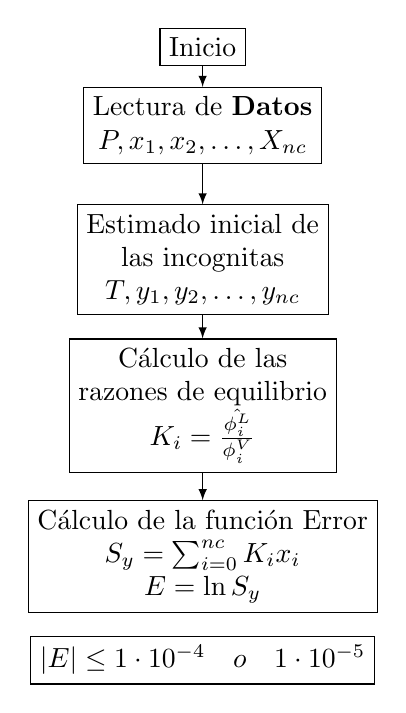
\begin{tikzpicture}[nodes={draw, fill=white,align=center},row sep=0.3cm,column sep=0.5cm] ]

\node(init){Inicio};
\node[below of=init] (lab)  {Lectura de \textbf{Datos} \\$P,x_1, x_2,\ldots, X_{nc}$};
\node[below of=lab,below](estim){Estimado inicial de\\ las incognitas\\$T,y_1,y_2,\ldots,y_{nc}$};
\node[below of=estim,below](relations){Cálculo de las\\ razones de equilibrio\\
$K_i = \frac{ \hat{\phi_i^L} }{ \phi_i^V}$};
\node[below of=relations,below = 0.2cm](error){Cálculo de la función Error\\$ S_y =\sum_{i=0}^{nc} K_i x_i $\\$ E = \ln{S_y} $};

\node[below of=error,below](criteria){$|E| \leq 1\cdot10^{-4}\quad \text{o} \quad  1\cdot 10^{-5}$};

\draw[-latex] (init)--(lab);
\draw[-latex] (lab)--(estim);
\draw[-latex] (estim)--(relations);
\draw[-latex] (relations)--(error);

\end{tikzpicture}

		\subsection{Temperatura de Rocío}\label{subsec:dewtemperature}

	El cálculo de temperatura de rocío para una mezcla se realiza como se indica en la figura \ref{fig:dewtemperature}. Usando un objeto del tipo `HeterogeneousMixture' de la librería \Materia el cálculo se realiza como se muestra en los fragmentos de código \ref{lst:dewtemperature} y \ref{lst:dewtemperatureWithEstimate}.

	Si al método no se le proporciona un estimado inicial, como se muestra en el código \ref{lst:dewtemperature} entonces la clase realiza la estimación de la temperatura como se muestra en la figura \ref{fig:dewtemperatureEstimate}. 

	\begin{lstlisting}[label={lst:dewtemperatureWithEstimate},caption={Cálculo de la temperatura de rocío proporcionando un estimado inicial.}]

		heterogeneousMixture.setZFraction(compound1,molarFraction1);
		//...... asignar la fracción molar para todos los compuestos

		heterogeneousMixture.setPressure(pressure);
		heterogeneousMixture.dewTemperature(temeperatureEstimate,liquidEstimatedFractions);
		double temperature = heterogeneousMixture.getTemperature();
	\end{lstlisting}


	\begin{lstlisting}[label={lst:dewtemperature},caption={Cálculo de la temperatura de rocío.}]

		heterogeneousMixture.setZFraction(compound1,molarFraction1);
		//...... asignar la fracción molar para todos los compuestos

		heterogeneousMixture.setPressure(pressure);
		heterogeneousMixture.dewTemperature();
		double temperature = heterogeneousMixture.getTemperature();
	\end{lstlisting}


		\subsection{Presión de Burbuja}\label{subsec:bubblepressure}

	El cálculo de presión de burbuja para una mezcla se realiza como se indica en la figura \ref{fig:bubblepressure}. Usando un objeto del tipo `HeterogeneousMixture' de la librería \Materia el cálculo se realiza como se muestra en los fragmentos de código \ref{lst:bubblepressure} y \ref{lst:bubblepressureWithEstimate}.

	Si al método no se le proporciona un estimado inicial, como se muestra en el código \ref{lst:bubblepressure} entonces la clase realiza la estimación de la presión de vapor con la ecuación del factor acéntrico \ref{eq:pressureacentricfactor}. 



	\begin{lstlisting}[label={lst:bubblepressureWithEstimate},caption={Cálculo de la presión de burbuja proporcionando un estimado inicial.}]

		heterogeneousMixture.setZFraction(compound1,molarFraction1);
		//...... asignar la fracción molar para todos los compuestos

		heterogeneousMixture.setTemperature(temperature);
		heterogeneousMixture.bubblePressure(
					pressureEstimate,vaporEstimatedFractions);
		double pressure = heterogeneousMixture.getPressure();
	\end{lstlisting}


	\begin{lstlisting}[label={lst:bubblepressure},caption={Cálculo de la presión de burbuja.}]
		heterogeneousMixture.setZFraction(compound1,molarFraction1);
		//...... asignar la fracción molar para todos los compuestos

		heterogeneousMixture.setTemperature(temperature);
		heterogeneousMixture.bubblePressure();
		double pressure = heterogeneousMixture.getPressure();
	\end{lstlisting}

	La figura \ref{fig:bubblepressure3d} muestra los planos obtenidos del líquido saturado y del vapor saturado por medio del cálculo de presión de burbuja para el sistema metanol-agua con la ecuación de PRSV.

\begin{figure}[p]
\centering
	\begin{tikzpicture}
	\begin{axis}[view/v=-15,colorbar left,xlabel={Fracción Molar del metanol},ylabel=\temperature,zlabel=\pressure,colorbar style={ylabel=\temperature,
        yticklabel style={
            text width=2.5em,
            align=right}}]
		\addplot3[surf,point meta=explicit,shader=interp]table[meta=temperature, y=temperature , x=liquidFraction, z=pressure]{plotdata/mixhet/hp.dat};
		\addplot3[surf,point meta=explicit,shader=interp]table[meta=temperature, y=temperature , x=vaporFraction, z=pressure]{plotdata/mixhet/hp.dat};
	\end{axis}
	\end{tikzpicture}


	\begin{tikzpicture}
	\begin{axis}[view/v=-220,xlabel={Fracción Molar del metanol},ylabel=\temperature,zlabel=\pressure]
	\addplot3[surf,point meta=explicit,shader=interp]table[meta=temperature, y=temperature , x=liquidFraction, z=pressure]{plotdata/mixhet/hp.dat};
	\addplot3[surf,point meta=explicit,shader=interp]table[meta=temperature, y=temperature , x=vaporFraction, z=pressure]{plotdata/mixhet/hp.dat};
	\end{axis}
	\end{tikzpicture}


	\begin{tikzpicture}
	\begin{axis}[view/v=-115,xlabel={Fracción Molar del metanol},ylabel=\temperature,zlabel=\pressure]
	\addplot3[surf,point meta=explicit,shader=interp]table[meta=temperature, y=temperature , x=liquidFraction, z=pressure]{plotdata/mixhet/hp.dat};
	\addplot3[surf,point meta=explicit,shader=interp]table[meta=temperature, y=temperature , x=vaporFraction, z=pressure]{plotdata/mixhet/hp.dat};
	\end{axis}
	\end{tikzpicture}
	\caption{Diagramas tridimensionales de presión-composición-temperatura para el sistema metanol-agua. En la figura podemos observar los planos formados por el líquido y el vapor saturado obtenidos con el cálculo de presión de burbuja. Los diagramas son la misma figura vista desde diferentes angulos.}\label{fig:bubblepressure3d}
\end{figure}

		\subsection{Presión de Rocío}\label{subsec:dewpressure}

	El cálculo de presión de rocío para una mezcla se realiza como se indica en la figura \ref{fig:dewpressure}. Usando un objeto del tipo `HeterogeneousMixture' de la librería \Materia el cálculo se realiza como se muestra en los fragmentos de código \ref{lst:dewpressure} y \ref{lst:dewpressureWithEstimate}.

	Si al método no se le proporciona un estimado inicial, como se muestra en el código \ref{lst:dewpressure} entonces la clase realiza la estimación de la presión de vapor con la ecuación del factor acéntrico \ref{eq:pressureacentricfactor}. 

	\begin{lstlisting}[label={lst:dewpressureWithEstimate},caption={Cálculo de la presión de rocío proporcionando un estimado inicial.}]

		heterogeneousMixture.setZFraction(compound1,molarFraction1);
		//...... asignar la fracción molar para todos los compuestos

		heterogeneousMixture.setTemperature(temperature);
		heterogeneousMixture.dewPressure(pressureEstimate);
		double pressure = heterogeneousMixture.getPressure();
	\end{lstlisting}

	\begin{lstlisting}[label={lst:dewpressure},caption={Cálculo de la presión de rocío.}]

		heterogeneousMixture.setZFraction(compound1,molarFraction1);
		//...... asignar la fracción molar para todos los compuestos

		heterogeneousMixture.setTemperature(temperature);
		heterogeneousMixture.dewPressure();
		double pressure = heterogeneousMixture.getPressure();
	\end{lstlisting}

\begin{figure}[!h]
	\begin{tikzpicture}[nodes={draw, fill=white,align=center},row sep=0.3cm,column sep=0.5cm] ]

	\node(init){Inicio};
	\node[below of=init,below] (lab)  {Lectura de \textbf{Datos} \\$T,y_1, y_2,\ldots, y_{nc}$};
	\node[below of=lab,below=0.4](estim){Estimado inicial de\\ las incognitas\\$P,x_1,x_2,\ldots,x_{nc}$};
	\node[below of=estim,below=0.4](relations){Cálculo de las\\ razones de equilibrio\\
	$K_i = \frac{ \hat{\phi}_i^L }{ \hat{ \phi}_i^V}$};
	\node[below of=relations,below = 0.5cm](error){Cálculo de la función Error\\
	$ S_x =\sum_{i=1}^{nc}\frac{y_i}{ K_i} $\\$ E = S_x-1 $};

	\node[below of=error,below=0.4](criteria){$|E| \leq 1\cdot10^{-4}\quad \text{o} \quad  1\cdot 10^{-5}$};
	\node[below of=criteria,below=0.4](tempIncrement){Incrementer la temperatura\\$P^* = P + \Delta P$\\
	$\Delta P = 0.001  \quad \text{o} \quad 0.0001 K$};

	\node[below of=tempIncrement,below=0.4](relationsWithIncrement){Cálculo de las Razones\\ de Equilibrio con $P^*$\\$K_i^* = \frac{ \hat{\phi}_i^L }{\hat{\phi}_i^V}$};

	\node[right of=criteria	,right=2.2cm](end){Fin};


	\node[right of=tempIncrement, right=3cm](errorWithIncrement){Cálculo de la función Error \\ con $P^*$\\
	$ S_x^* =\sum_{i=1}^{nc} \frac{y_i}{K_i^*}  $\\$ E^* = S_x^*-1 $};

	\node[right of=relations, right = 3cm](newValues){Cálculo de las nuevas estimaciones \\ de las \textbf{Incógnitas}\\
	\begin{minipage}{0.2\linewidth}
	\begin{equation*}
	T_{nueva} =P- \frac{E  \left(P^*-P\right)}{E^*-E}
	\end{equation*}
	\begin{equation*}
	 S_x =\sum_{i=1}^{nc}\frac{y_i}{K_i}   \\
	 \end{equation*}
	 \begin{equation*}
	\left(x_i\right)_{nueva} = \frac{y_i}{K_i S_x}
	\end{equation*}
	\end{minipage}
	};


	\draw[-latex] (init)--(lab);
	\draw[-latex] (lab)--(estim);
	\draw[-latex] (estim)--(relations);
	\draw[-latex] (relations)--(error);
	\draw[-latex] (error)--(criteria);
	\draw[-latex] (criteria)--node[fill=none,draw=none,above]{SI}(end);
	\draw[-latex] (criteria)--node[fill=none,draw=none,left]{NO}(tempIncrement);
	\draw[-latex] (tempIncrement)--(relationsWithIncrement);
	\draw[-latex] (relationsWithIncrement)--(errorWithIncrement);
	\draw[-latex] (errorWithIncrement)--(newValues);
	\draw[-latex] (newValues)--(relations);

	\end{tikzpicture}
	\caption{Algoritmo para el cálculo de la presión de rocío.}\label{fig:dewpressure}
\end{figure}
		\subsection{Flash}



\begin{tikzpicture}[nodes={draw, fill=white,align=center},row sep=0.3cm,column sep=0.5cm] ]

\node(init){Inicio};
\node[below of=init] (lab)  {Lectura de \textbf{Datos} \\$T,P,z_1, z_2,\ldots, z_{nc}$};
\node[below of=lab,below](estim){Estimado inicial de\\ las incognitas\\$V/F,x_1,x_2,\ldots,x_{nc}$\\$y_1,y_2 \ldots, y_{nc}$};
\node[below of=estim,below](relations){Cálculo de las\\ razones de equilibrio\\
$K_i = \frac{ \hat{\phi}_i^L }{ \hat{ \phi}_i^V}$};
\node[below of=relations,below = 0.2cm](error){Cálculo de la función Error\\
$ \zeta =\sum_{i=1}^{nc}\left| x_i \hat{\varphi}_i^L - y_i \hat{\varphi}_i^V \right|$};

\node[below of=error,below](criteria){$|\zeta| \leq 1\cdot10^{-4}\quad \text{o} \quad  1\cdot 10^{-5}$};


\node[below of=criteria,below](rachford){Cálculo de $V/F$ con Rachford-Rice:\\ 
\begin{minipage}{0.5\linewidth}
\begin{equation*}
S = \sum_{i=1}^{nc}\frac{z_i\left(K_i - 1\right)}{1+ \frac{V}{F}\left(K_i-1\right)}
\end{equation*}
Encontrar $V/F$ tal que $S = 0$\\
Método de Newton-Raphson\\
\begin{equation*}
\acute{S} = \sum_{i=1}^{nc} \frac{-z_i \left(K_i - 1\right)^2}{\left[1+ \frac{V}{F} \left(K_i-1\right)\right]^2}
\end{equation*}
\begin{equation*}
\left(\frac{V}{F}\right)_{nueva} = \left(\frac{V}{F}\right) - \frac{S}{\acute{S}}
\end{equation*}
\end{minipage}};

\node[right of=criteria	,right=2.2cm](end){Fin};


\node[right of=estim, right = 3cm](newValues){Cálculo de las nuevas estimaciones \\ de las \textbf{Incógnitas}\\
\begin{minipage}{0.3\linewidth}
\begin{equation*}
\acute{x_i} = \frac{z_i}{1 + \frac{V}{F}\left(K_i-1\right)}
\end{equation*}
\begin{equation*}
 S_x =\sum_{i=1}^{nc}\acute{x}_i \qquad x_i = \frac{\acute{x_i}}{S_x}
\end{equation*}
\begin{equation*}
\acute{y_i} = \acute{x_i} K_i = \frac{z_i K_i}{1+\frac{V}{F}\left(K_i - 1\right)}
\end{equation*}
\begin{equation*}
 S_y =\sum_{i=1}^{nc}\acute{y}_i \qquad y_i = \frac{\acute{y_i}}{S_y}
\end{equation*}
\end{minipage}
};


\draw[-latex] (init)--(lab);
\draw[-latex] (lab)--(estim);
\draw[-latex] (estim)--(relations);
\draw[-latex] (relations)--(error);
\draw[-latex] (error)--(criteria);
\draw[-latex] (criteria)--node[fill=none,draw=none,above]{SI}(end);
\draw[-latex] (criteria)--node[fill=none,draw=none,left]{NO}(rachford);

\draw[-latex] (rachford)-|(newValues);
\draw[-latex] (newValues)--(relations);

\end{tikzpicture}

		\subsection{Diagramas}
	


		\section{Sistema de Unidades}

Las unidades que utiliza la librería se muestran en la tabla \ref{tab:units}.
Durante este escrito se utilizarán las mismas unidades, a menos que se indique lo contrario.


\begin{table}
\begin{tabular}{ |c| c|c|}
	\hline
		Propiedad & Unidad &\\
	\hline
		Presión & $Pa$ & Pascal\\
		Temperatura & $K$ & Kelvin\\
		Volumen molar & $\frac{m^3}{kg}$ & Metro cúbico sobre kilogramo\\

	\hline
\end{tabular}

\caption{Sistema de unidades empleado por la librería}\label{tab:units}
\end{table}%hecho
		\section{Ecuación de estado cúbica}

La ecuación de estado cúbica representada por la clase ``Cubic'', permite realizar los cálculos de: 
\begin{itemize}
\itemsep0ex
	\item{\nameref{subsec:pressure}} 
	\item{\nameref{subsec:compresibilityFactor}}
	\item{Volumen molar}
	\item{Fugacidad}
	\item{Adimensionalización de los parámetros a y b}
\end{itemize}

En la tabla \ref{tab:cubics} se muestran las ecuaciones implementadas en este trabajo.

 \subsection{Presión}
 \label{subsec:pressure}

Un cálculo de presión, se realiza como se muestra en el código \ref{lst:pressureCalculation}.
\begin{lstlisting}[label=lst:pressureCalculation,caption=Cálculo de presión para el heptano con la ecuación de estado cúbica de Van Der Waals]
import termo.eos.Cubic;
...
Cubic cubic = new Cubic();
//parametros de van der waals para el heptano
double a = 3107000.0;
double b = 0.2049;

double volume = 1.5;
double temperature = 300;
double pressure = cubic.calculatePressure(temperature, volume, a, b);
\end{lstlisting}

\begin{figure}
\begin{tabular}{c c}
	\begin{tikzpicture}
	\begin{axis}[width= 0.45 \linewidth,font=\footnotesize,
	xlabel = {Volumen molar $[\frac{m^3}{kg}]$},
	ylabel = {Presión $[Pa]$}]
	\addplot[blue]table{plotdata/pressurevolume.dat};
	\end{axis}
	\end{tikzpicture}
	&
	\begin{tikzpicture}
	\begin{axis}[width= 0.45 \linewidth,,font=\footnotesize,
	xlabel={Volumen molar $[\frac{m^3}{kg}]$},
	zlabel={Presión $[Pa]$},
	ylabel={Temperatura $[K]$}]
	\addplot3[surf,
	colormap={blueblack}{color=(white) color=(blue)},
	domain=0:1]table{plotdata/pressurevolumetemperature.dat};
	\end{axis}
	\end{tikzpicture}
\end{tabular}
\caption{Diagramas de presión usando la eq. de Van Der Waals (u=w=0)} \label{fig:cubicPressureDiagrams}
\end{figure}


De manera predeterminada los valores u y w de la ecuación de estado son iguales a 0. En la figura \ref{fig:cubicPressureDiagrams} se muestra un ejemplo de uso del cálculo para realizár gŕaficas de presión.

Podemos asignar los valores u y w para la ecuación de estado cúbica, o podemos utilizar la clase ``EquationsOfState'' para obtener una ecuación con los parámetros previamente establecidos, los fragmentos de código \ref{lst:pengRobinsonCreation} y \ref{lst:tstCreation} muestran el procedimiento respectivamente.

\begin{lstlisting}[label=lst:pengRobinsonCreation,caption=Creación de la ecuación de estado de Peng Robinson usando los metodos `Set' de los parametros u y w]
Cubic pengRobinson = new Cubic();
pengRobinson.setU(2);
pengRobinson.setW(-1);
\end{lstlisting}

\begin{lstlisting}[label=lst:tstCreation,caption=Creación de la ecuación de estado de TST usando la clase EquationsOfState]
Cubic tst = EquationsOfState.twoSimTassone();
\end{lstlisting}












%hecho
		\subsection{Factor de compresibilidad}

Solución de la ecuación de estado cúbica

\begin{equation}
p=\frac{RT}{v-b} - \frac{a}{v^2 + ubv+ wb^2}
\qquad
A=\frac{ap}{(RT)^2}
\qquad
B=\frac{bp}{RT}
\end{equation}

\begin{equation}
z^3-\left[1-(u-1)B\right]z^2+ \\ \left[A-uB-uB^2 +\\ wB^2\right]z-\left[AB+wB^2+wB^3\right]=0
\end{equation}


\begin{align}
\alpha &= 1-(u-1)B\\
\beta &= A -uB-uB^2+wB^3\\
\gamma &= AB +wB^2+ 2B^3\\
C &= 3\beta - \alpha^2\\
D&= - \alpha^3+ 4.5 \alpha \beta -13.5 \gamma\\
Q&=C^3+D^2
\end{align}


\begin{itemize}
\item Si $Q \leq 0 \qquad \vartheta = \arccos \left[\frac{-D}{\sqrt{-C^3}}\right]$
\begin{description}
\item{Líquido} $z = \frac{1}{3}\left[\alpha + 2 \sqrt{-C} \cos\left(\frac{\vartheta}{3} + 120\degree \right)\right]$
\item{Vapor} $z = \frac{1}{3}\left[\alpha + 2 \sqrt{-C} \cos\left(\frac{\vartheta}{3}\right)\right]$
\end{description}
Nota: En caso de que el z del líquido sea menor que B, entonces hay que calcularla como si fuera vapor.
\item Si $Q > 0 \qquad z = \frac{1}{3}\left[\alpha + \left(-D + \sqrt{Q}\right)^{\frac{1}{3}}+ \left(-D - \sqrt{Q}\right)^{\frac{1}{3}} \right]$
\end{itemize}



\begin{tikzpicture}
\begin{axis}
\addplot[blue]table{plotdata/compresibilitiChart/pz_temp_1.dat};
\addplot[blue]table{plotdata/compresibilitiChart/pz_temp_2.dat};
\addplot[blue]table{plotdata/compresibilitiChart/pz_temp_3.dat};
\addplot[blue]table{plotdata/compresibilitiChart/pz_temp_4.dat};
\addplot[blue]table{plotdata/compresibilitiChart/pz_temp_5.dat};
\addplot[blue]table{plotdata/compresibilitiChart/pz_temp_6.dat};
\addplot[blue]table{plotdata/compresibilitiChart/pz_temp_7.dat};
\addplot[blue]table{plotdata/compresibilitiChart/pz_temp_8.dat};
\addplot[blue]table{plotdata/compresibilitiChart/pz_temp_9.dat};
\addplot[blue]table{plotdata/compresibilitiChart/pz_temp_10.dat};
\end{axis}
\end{tikzpicture}

%hecho
		\subsection{Parámetros de la ecuación de estado cúbica}


Existen dos formas para calcular los parámetros de la ecuación dependiendo de la cantidad de compuestos presentes en el sistema a estudiar.
\begin{itemize}
 \item Compuesto puro
 \item Mezcla. 
\end{itemize}

La clase "Substance" realiza los cálculos para los compuestos puros, mientras que la clase "Mixture" realiza los cálculos para la mezcla. Una vez obtenido el cálculo de los parámetros la super clase "Homogeneous" utiliza los parámetros para realizar el cálculo de propiedades.

\begin{lstlisting}[caption=Cualquier objeto tipo Homogeneous puede calcular los parámetrod de la ecuación de estado cúbica a y b]
	Homogeneous system = ....
	double a = system.calculate_a_cubicParameter();
	double b = system.calculate_b_cubicParameter();
\end{lstlisting}


La estructura de la librería se muestra en \ref{fig:homogeneousCalculations}

\begin{figure}[!h]
  
  \centering
    \includegraphics[scale=0.7]{homogeneousCalculations.png}
    \caption{A picture of a gull.}
    \label{fig:homogeneousCalculations}
\end{figure}

\subsection{Compuesto puro}
Los parámetros para un compuesto puro dependen de la ecuación de estado cúbica y de una expresión $\alpha$ .

\begin{equation}
	b_i = \Omega_b \frac{R T_{ci}}{p_{ci}} 
\end{equation}

\begin{equation}
 a_i = \Omega_a \frac{\left(R T_{ci}\right)^2}{p_{ci}} \alpha_i
\end{equation}

La expresión de $\alpha$ puede ser una función de la temperatura.

\begin{table}
\begin{tabular}{|c |c|c| }
	\hline
	Expresión & Parámetros & Ecuación de estado\\
	\hline
	Soave    &  ---& PR\\
	Peng and Robinson & ---& PR \\
	Mathias & $A$ & SRK\\
	Stryjek and Vera & $k_1$ & PRSV\\
	Adachi and Lu & $A,B$&SRK,PR\\
	Soave & $A,B$&SRK,PR\\
	Melhem, et al. & $A,B$&SRK,PR\\
	Androulakis et al. & $A,B,C$& SRK,PR\\
	Mathias and Copeman & $A,B,C$& SRK,PR\\
	Yu and Lu & $A,B,C$&SRK,PR\\
	Stryjek and Vera & $A,B,C$&PR\\
	Twu & $L,M,N$&TST\\
	Twu & ---&TST,PR\\
	GCEOS & ---& (Cualquier u y w)\\
	\hline
\end{tabular}
\caption{Expresiónes de $\alpha$ disponibles en la librería}\label{tab:alphas}
\end{table}


Para realizar el cálculo de los parámetros de la ecuación para el compuesto i, es necesario elegir la ecuación de estado cúbica (u,w, $\Omega_a$ y $\Omega_b$) y la expresión de $\alpha$.

En la sección \ref{subsec:pressure} se mostró como crear una ecuación de estado cúbica y asignar las variables $u$ y $w$. De igual manera podemos asignar el valor de $\Omega_a$ y $\Omega_b$ \footnote{Los valore de $\Omega_a$ y $\Omega_b$ se muestran en la tabla \ref{tab:cubics}}, o elegir la ecuación de estado cúbica previamente definida, a través de la clase ``EquatiosOfState''. Por comodidad usaremos la segunda aproximación.

Se debe elegir la expresión de $\alpha$ de la clase Alphas \footnote{Las expresiones de $\alpha$ disponibles se listan en \ref{tab:alphas}}. Es posible crear o modificar una expresión de $\alpha$, pero debido a su complejidad sera tratado en una sección aparte.

Para realizar el cálculo es necesario definir las propiedades del compuesto, temperatura crítica, presión crítica, y algunas expresiones de $\alpha$ necesitan el factor acéntrico, para lo cual existe la clase Compound que encapsula todas las propiedades del compuesto.



\begin{lstlisting}[caption=Cálculo de los parámetros de la ecuación de estado Soave Redlich Kwong y la expresión de $\alpha$ de mathias para el compuesto ]
import.termo.eos.Cubic;
...
Compound compound = new Compound("Cyclohexane");
compound.setCriticalPressure(4073000);
compound.setCriticalTemperature(553.5);
compound.setAcentricFactor(0.211);

Cubic srk = EquationsOfState.redlichKwongSoave();
Alpha mathias = Alphas.getMathiasExpression();

Substance substance = new Substance(srk,mathias, compound,Phase.LIQUID);

double a = substance.calculate_a_cubicParameter();
double b = substance.calculate_b_cubicParameter();
\end{lstlisting}





\subsubsection{Mezcla}

El cálculo de los parámetros para una mezcla depende de la regla de mezclado.Para las reglas de mezclado basadas en la energía libre de Gibbs de exceso el cálculo también depende del modelo de actividad elegido.

\begin{tabularx}{\textwidth}{|X|X|X|}
	\hline
	Regla & Parámetros & \\
	\hline
	Van Der Waals & $k_{ij}$ & $k_{ij} = k_{ji}$ \\
	Mathias-Klotz-Prausnitz& $k_{ij}$ & $k_{ij} \neq k_{ji}$ \\
	Basadas en la energía libre de Gibbs de exceso. & Segun el modelo de actividad y la implementación de la regla.& --- \\
	\hline
\end{tabularx}



\begin{lstlisting}[caption=Código para el cálculo de los parámetros de la ecuación de estado en una mezcla. ]
import termo.component.Compound;
import termo.eos.Cubic;
import termo.eos.EquationsOfState;
import termo.eos.alpha.Alpha;
import termo.eos.alpha.Alphas;
import termo.matter.Mixture;
import termo.matter.Substance;
import termo.matter.factory.MixtureBuilder;
import termo.phase.Phase;
...
Compound cyclohexane = new Compound("Cyclohexane");
cyclohexane.setCriticalPressure(4073000);
cyclohexane.setCriticalTemperature(553.5);
cyclohexane.setAcentricFactor(0.211);

Compound pentane = new Compound("N-pentane");
pentane.setCriticalPressure(3370000);
pentane.setCriticalTemperature(469.7);
pentane.setAcentricFactor(0.251);

Cubic equationOfState = EquationsOfState.pengRobinson();
Alpha alpha = Alphas.getMathiasAndCopemanExpression();

Mixture mixture = new MixtureBuilder()
			.addCompounds(cyclohexane,pentane)
			.setAlpha(alpha)
			.setEquationOfState(equationOfState)
			.setPhase(Phase.VAPOR)
			.build();

double a = mixture.calculate_a_cubicParameter();
double b = mixture.calculate_b_cubicParameter();
\end{lstlisting}


Si se requiere utilizar una expresión de $\alpha$ diferente para cada compuesto.
\begin{lstlisting}
Mixture mixture = new MixtureBuilder()
			.addCompound(cyclohexane,Alphas.getPengAndRobinsonExpression())
			.addCompound(pentane,Alphas.getStryjekAndVeraExpression())
			.setEquationOfState(eos)
			.setPhase(phase)
			.setMixingRule(mixingRule)
			.setInteractionParameter(k)
			.build();

double a = mixture.calculate_a_cubicParameter();
double b = mixture.calculate_b_cubicParameter();
\end{lstlisting}
%hecho

		\subsection{Entalpía}

\begin{equation}
h = h^{\neq} + \left[ \frac{T(\frac{\partial a}{\partial T}) - a}{b\sqrt{u²-4w} }\right] 
\ln\left[\frac{2v+b\left(u + \sqrt{u²-4w}\right)}{2v+b\left(u - \sqrt{u²-4w}\right)}\right]
+ pv - RT
\end{equation}

\begin{lstlisting}[label=some-code,caption=Some Code]
private  double calculateEnthalpy( double volume){
    double idealGasEnthalpy = calculateIdealGasEnthalpy();
    double a = calculate_a_cubicParameter();
    double b = calculate_b_cubicParameter();
    double L = cubicEquationOfState.calculateL(volume, b);
    double partial_aPartial_temperature = partial_aPartial_temperature( );
    
    return idealGasEnthalpy + ((partial_aPartial_temperature - a)/b) * L  + pressure * volume - Constants.R *temperature;
}
\end{lstlisting}	


\subsubsection{Entalpía del gas ideal}
\begin{equation}
h^{\neq} = \sum_{i=1}^{nc} x_i \left[ h_i^{ref} + \int_{Tref}^{T} Cp_i^{\neq} \mathrm{d}T \right]
\end{equation}



\begin{tikzpicture}
\begin{axis}
\addplot[blue]table{plotdata/enthalpy/lv.dat};
\end{axis}
\end{tikzpicture}

\begin{tikzpicture}
\begin{axis}[view/h=-165]
\addplot3[surf]table{plotdata/enthalpy/lv3d.dat};
\addplot3[surf]table{plotdata/enthalpy/l3d.dat};
\addplot3[surf]table{plotdata/enthalpy/v3d.dat};
\end{axis}
\end{tikzpicture}
\begin{tikzpicture}
\begin{axis}[view/h=-225]
\addplot3[surf]table{plotdata/enthalpy/lv3d.dat};
\addplot3[surf]table{plotdata/enthalpy/l3d.dat};
\addplot3[surf]table{plotdata/enthalpy/v3d.dat};
\end{axis}
\end{tikzpicture}
\begin{tikzpicture}
\begin{axis}[view/h=-120]
\addplot3[surf]table{plotdata/enthalpy/lv3d.dat};
\addplot3[surf]table{plotdata/enthalpy/l3d.dat};
\addplot3[surf]table{plotdata/enthalpy/v3d.dat};
\end{axis}
\end{tikzpicture}	

		
		\subsection{Expresiones de $\alpha$}

	\input{calculatingProperties/alpha/soave}
	\subsubsection{Peng and Robinson \cite{pengRobinson}}


\begin{gather}
	\alpha^{\nicefrac{1}{2}} = 1 + m \left(1-\sqrt{T_r}\right)\\
	m = 0.37464+1.54226\omega-0.2699\omega^2
\end{gather}
	\subsubsection{Mathias\cite{mathias} }
\begin{itemize}

\item{$T < T_C$}
\begin{gather}
	\alpha^{\nicefrac{1}{2}} = 1 + m \left(1-\sqrt{T_r}\right)- A\left(1-T_r\right)\left(0.7-T_r\right)
	\\
	m = 0.48508+1.55191\omega-0.15613\omega^2
\end{gather}

\item{$T > T_c$}
\begin{gather}
	\alpha = \exp{\left[ \left( \frac{c-1}{c} \right)  \left(  1- T_r^c  \right)  \right]}\\
	c = 1 + \frac{m}{2} + 0.3 A
\end{gather}

 \end{itemize}


	\subsubsection{Stryjek and Vera(PRSV)\cite{stryjekVeraPureCompounds} }
\begin{itemize}

\item{$T < T_C$}
\begin{gather}
	\alpha^{\nicefrac{1}{2}} = 1 + \kappa_0 \left(1-\sqrt{T_r}\right)- \kappa_1\left(1-T_r\right)\left(0.7-T_r\right)
	\\
	\kappa_0 = 0.378893+1.4897153\omega-0.17131848\omega^2+0.0196554\omega³
\end{gather}

\item{$T > T_c$}
\begin{equation}
	\alpha^{\nicefrac{1}{2}} = 1 + \kappa_0\left(1- \sqrt{T_r}\right)
\end{equation}

 \end{itemize}	
	\subsubsection{Adachi and Lu \cite{adachiLu}}

\begin{equation}
\alpha = A\cdot {10}^{B\left(1-T_r\right)}
\end{equation}
	\subsubsection{Soave \cite{soaveR}}

\begin{equation}
\alpha= 1+\left(1-T_r\right)\left(A + \frac{B}{T_r}\right)
\end{equation}
	\subsubsection{Melhem, et al.\cite{melhem}}

\begin{equation}
\ln{\alpha}=A\left(1-T_r\right)+ B\left(1-\sqrt{T_r}\right)^2
\end{equation}
	\subsubsection{Androulakis,et al.\cite{androulakis}}

\begin{itemize}
\item{$T < T_C$}
\begin{equation}
 \alpha = 1 + A \left(1-T_r^{\nicefrac{2}{3}}\right) + B\left(1-T_r^{\nicefrac{2}{3}}\right)^2+ C\left(1-T_r^{\nicefrac{2}{3}}\right)^3
\end{equation}
\item{$T > T_c$}
\begin{equation}
\alpha = \mathrm{e}^{A\left(1-T_r^{\nicefrac{2}{3}}\right)}
\end{equation}
\end{itemize}
	\subsubsection{Mathias and Copeman. \cite{mathiasCopeman,michelsen}}

\begin{itemize}
\item{$T < T_c$}
\begin{equation}
\alpha^{\nicefrac{1}{2}} = 1 + A\left(1-\sqrt{T_r}\right) + B\left(1-\sqrt{T_r}\right)^2 + C\left(1-\sqrt{T_r}\right)^3
\end{equation}
\item{$T > T_c$}
\begin{equation}
\alpha^{\nicefrac{1}{2}} = 1 + A\left(1-\sqrt{T_r}\right)\footnote{La ecuación no se incluyó en el trabajo original de Mathias and Copeman\cite{mathiasCopeman}; esta expresión fue incorporada en el trabajo de Dahl and Michelsen \cite{michelsen}}
\end{equation}
\end{itemize}
	\subsubsection{Yu and Lu\cite{yuLu}}

\begin{itemize}
\item{$T < T_c$}
\begin{equation}
 \log_{10}{\alpha} = \left(A+B T_r+ C T_r^2\right)\left(1-T_r\right)
\end{equation}
\item{$T > T_c$}
\begin{equation}
 \log_{10}{\alpha} = \left(A+B+C \right)\left(1-T_r\right)
\end{equation}
\end{itemize}
	\subsubsection{Stryjek and Vera\cite{stryjekVera}}

\begin{itemize}
\item{$T < T_c$}
\begin{gather}
\alpha^{\nicefrac{1}{2}} = 1 + \kappa\left(1-\sqrt{T_r}\right)\\
\kappa = m + \left[
		A+ B\left(C- T_r\right)\left(1-\sqrt{T_r}\right)
	\right]
	\left[
		\left(1+ \sqrt{T_r}\right)\left(0.7-T_r\right)
	\right]\\
m=0.378893 + 1.4897153 \omega - 0.17131848 \omega^2+ 0.0196554 \omega^3
\end{gather}
\item{$T > T_c$}
\begin{equation}
\alpha^{\nicefrac{1}{2}} = 1 + m\left(1-\sqrt{T_r}\right)
\end{equation}
\end{itemize}
	\subsubsection{Twu\cite{twuequation}}
\begin{equation}
	\alpha = T_r^{N\left(M-1\right)}\exp{\left(L\left(1-T_r^{N M}\right)\right)}
\end{equation}
	\subsubsection{Twu \cite{twuactivity}}
\begin{itemize}
\item{$T < T_c$}
\begin{gather}
\alpha = \alpha^{(0)} + \omega\left(\alpha^{(1)}-\alpha^{(0)}\right)\\
\text{Para}\qquad \alpha^{(0)}\notag\\
L= 0.196545\qquad M=0.906437\qquad N=1.26251\\
\text{Para}\qquad \alpha^{(1)}\notag\\
L=0.704001 \qquad M =0.790407 \qquad N=2.13076
\end{gather}
\item{$T > T_c$}
\begin{gather}
\alpha = \alpha^{(0)} + \omega\left(\alpha^{(1)}-\alpha^{(0)}\right)\\
\text{Para}\qquad \alpha^{(0)}\notag\\
L= 0.358826\qquad M=4.23478\qquad N=-0.2\\
\text{Para}\qquad \alpha^{(1)}\notag\\
L=0.0206444 \qquad M =1.22942 \qquad N=-8.0
\end{gather}
\end{itemize}
	\subsubsection{GCEOS (AspenHYSYS)}

\begin{gather}
\alpha^{\nicefrac{1}{2}} = 1 + \kappa \left(1 - \sqrt{T_r}\right)\\
\kappa = \kappa_0 + \left[ 
	\kappa_1 + \left(   \kappa_2 - \kappa_3 T_r   \right)
	\left(1 - T_r^{\kappa_4}\right) 
\right]
\left[
	\left(1 + \sqrt{T_r}\right)\left(0.7 - T_r\right)
\right]
T^{\kappa_5}\\
\kappa_0 = A + B \omega+ C \omega^2+ D \omega^3
\end{gather}





\begin{equation}
P = \frac{R T}{v-b} - \frac{a}{v^2 +u b v + w b^2 }
\end{equation}


\begin{itemize}\itemsep0ex
\item $P$ : presión en $[Pa]$.
\item $v$ : volumen molar en $[\frac{m^3}{kg}]$
\item $a$ : Es una medida de la atracción entre las partículas. $[\frac{m^5}{kg s}]$
\item $b$ : volumen excluido por un mol de partículas.$[\frac{m^3}{kg}]$
\item $u$ y $w$ : Son los parámetros diferentes para cada ecuación de estado, ver tabla \ref{tab:cubics}
\item $R$ : Constante universal de los gases ideales en $\frac{m^3 Pa}{kgmol K}$
\end{itemize}

	\begin{table}
	
	\begin{tabular}{|c |c | c | c | c |}
		\hline
		Ecuación de estado  & $u$ & $w$ & $\Omega_a$&$\Omega_b$\\
		\hline
		Van Der Waals  & $0$ & $0$ & $0,421875$ & $0,125$\\
		\hline
		Peng robinson  & $2$ & $-1$ & $0.45723553$ & $0.077796074$\\
		\hline
		Redlich Kwong  & $1$ & $0$ & $0.42748023$ & $0.08664035$\\
		\hline
		TST  & $2.5$ & $-1.5$ &$ 0.470507$ & $0.0740740$\\
		\hline
	\end{tabular}
	\caption{Ecuaciónes de estado cúbicas}\label{tab:cubics}
	\end{table}





\begin{equation}
z= \frac{P V}{R T}
\qquad
A=\frac{ap}{(RT)^2}
\qquad
B=\frac{bp}{RT}
\end{equation}

\begin{equation}
z^3-\left[1-(u-1)B\right]z^2+ \\ \left[A-uB-uB^2 +\\ wB^2\right]z-\left[AB+wB^2+wB^3\right]=0
\end{equation}
		
		\subsection{Fugacidad}\label{subsec:fugacity}
	
	El cálculo de fugacidad se realiza para un compuesto en específico. Si el cálculo se desea hacer para una mezcla homogénea, será necesario especificar el compuesto para el cual se desea la fugacidad.Si el cálculo es para una substancia no será necesario especificar el compuesto, ya que la substancia solo tiene un compuesto puro. En el código \ref{lst:substancefugacity} se realiza el cálculo de fugacidad para una substancia, y en el código \ref{lst:mixturefugacity} se realiza el cálculo de fugaciad para un compuesto en una mezcla.

\begin{lstlisting}[label={lst:substancefugacity}, caption={Cálculo de la fugacidad para una substancia homogénea.}]
	double fugacity = substance.calculateFugacity();
\end{lstlisting}

\begin{lstlisting}[label={lst:mixturefugacity}, caption={Cálculo de la fugacidad para un compuesto en una mezcla.}]
	double fugacity = mixture.calculateFugacity(compound);
\end{lstlisting}

	Para crear la figura \ref{fig:fugacity} se calculó la fugacidad de una substancia en su fase vapor, y despues en su fase líquida, los planos se cruzan en la línea de equilibrio Líquido-Vapor.

\begin{figure}
	\centering
	\begin{tikzpicture}
	\begin{axis}[view/h=-170,view/v=15,xlabel={Temperatura $[K]$},ylabel={Presión $[Pa]$},zlabel={Fugacidad},width=0.6\linewidth,smooth,
	every axis y label/.style={at={(current axis.south east)},right=2mm},]
	\addplot3[surf,point meta=explicit,shader=interp]table[meta=temperature, z=liquidfug , x=temperature,y=pressure]{plotdata/fugacity/fug3d.dat};
	\addplot3[surf,point meta=explicit,shader=interp]table[meta=temperature, z=vaporfug , x=temperature,y=pressure]{plotdata/fugacity/fug3d.dat};
	\addplot3[point meta=explicit]table[meta=temperature, z=fug , x=temperature,y=pressure]{plotdata/fugacity/linefug3d.dat};
	\end{axis}
	\end{tikzpicture}
	\caption{La fugacidad del líquido y del vapor coinciden en la línea de equilibrio.}\label{fig:fugacity}
\end{figure}




		
		\subsection{Entropía}

	El cálculo de la entropía es muy semejante al de la entalpía, es necesario conocer la entropía del gas ideal y la entropía residual.

\subsubsection{Entropía del gas ideal}

	El cálculo de la entropía segun el gas ideal, también necesita una ecuación que represente capacidad calorífica. En la sección \ref{sec:cp} se muestran las ecuaciónes de $C_p$ incluidas en la librería y como usarlas.

	En el fragmento de código \ref{lst:idealgasentropy} se muestra el cálculo de la entropía del gas ideal según la ecuación \ref{eq:idealgasentropy}. 

	\begin{lstlisting}[label={lst:idealgasentropy},caption={Cálculo de la entropía absoluta del gas ideal.}]
	double idealGasEntropy = homogeneous.calculateIdealGasEntropy();
	\end{lstlisting}

\subsubsection{Entropía real}

	El cálculo de la entalpía se realiza según la ecuación \ref{eq:entropy} y su uso se muestra en el código \ref{lst:entropy}.

\begin{lstlisting}[label={lst:entropy},caption={Cálculo de la entropía absoluta.}]
	double entropy = homogeneous.calculateEntropy()
\end{lstlisting}

	Las figuras \ref{fig:2dentropy} y \ref{fig:entropy3d} muestran diagramas de entalpía creados con ayuda de la librería \Materia.


\begin{figure}[!h]
	\centering	
	\begin{tikzpicture}
	\begin{axis}[xlabel={\entropy},ylabel=\pressure]
	\addplot[blue]table{plotdata/entropy/lv.dat};
	\end{axis}
	\end{tikzpicture}
	\caption{Diagrama de presión-entropía para el agua. Las líneas azules representan isotermas.}\label{fig:2dentropy}
\end{figure}


%	\begin{tikzpicture}
%	\begin{axis}[view/h=-45,xlabel={\entropy},ylabel={\molarVolume},zlabel={\pressure},colorbar]
%	\addplot3[surf,point meta=explicit]table[meta=temperature,x=pressure,y=entropy,z=temperature]{plotdata/entropy/lv3d.dat};
%	\addplot3[surf,point meta=explicit]table[meta=temperature,x=pressure,y=entropy,z=temperature]{plotdata/entropy/l3d.dat};
%	\addplot3[surf,point meta=explicit]table[meta=temperature,x=pressure,y=entropy,z=temperature]{plotdata/entropy/v3d.dat};
%	\end{axis}
%	\end{tikzpicture}

\begin{figure}[!h]
	\begin{tikzpicture}
	\begin{axis}[view/h=-165,xlabel={\entropy},ylabel={\molarVolume},zlabel={\pressure},colorbar,colorbar style={ylabel=Temperatura (K),title=Código de color}]
	\addplot3[surf,point meta=explicit]table[meta=temperature]{plotdata/entropy/lv3d.dat};
	\addplot3[surf,point meta=explicit]table[meta=temperature]{plotdata/entropy/l3d.dat};
	\addplot3[surf,point meta=explicit]table[meta=temperature]{plotdata/entropy/v3d.dat};
	\end{axis}
	\end{tikzpicture}
	% \begin{tikzpicture}
	% \begin{axis}[view/h=-225,xlabel={\entropy},ylabel={\molarVolume},zlabel={\pressure}]
	% \addplot3[surf,point meta=explicit]table[meta=temperature]{plotdata/entropy/lv3d.dat};
	% \addplot3[surf,point meta=explicit]table[meta=temperature]{plotdata/entropy/l3d.dat};
	% \addplot3[surf,point meta=explicit]table[meta=temperature]{plotdata/entropy/v3d.dat};
	% \end{axis}
	% \end{tikzpicture}
	% \begin{tikzpicture}
	% \begin{axis}[view/h=-120,xlabel={\entropy},ylabel={\molarVolume},zlabel={\pressure}]
	% \addplot3[surf,point meta=explicit]table[meta=temperature]{plotdata/entropy/lv3d.dat};
	% \addplot3[surf,point meta=explicit]table[meta=temperature]{plotdata/entropy/l3d.dat};
	% \addplot3[surf,point meta=explicit]table[meta=temperature]{plotdata/entropy/v3d.dat};
	% \end{axis}
	% \end{tikzpicture}
	\caption{Diagramas tridimensional presión-entropía-`volumen molar' para el agua.}\label{fig:entropy3d}
\end{figure}
		\subsection{Energía libre de Gibbs}
	
	El cálculo de la energía libre de Gibbs se realiza a partir de la entropía y la entalpía segun la ecuación \ref{eq:gibbs} y su cálculo se demuestra en el código \ref{lst:gibbs}.

	\begin{lstlisting}[label={lst:gibbs},caption={Cálculo de la energía libre de Gibbs con la librería \Materia}]
		double gibbs = homogeneous.calculateGibbs();
	\end{lstlisting}

	Las figuras \ref{fig:2dgibbs} y \ref{fig:gibbs3d} muestran diagramas de la energía libre de Gibbs creados con ayuda de la librería \Materia.

\begin{figure}[!h]
	\centering	
	\begin{tikzpicture}
	\begin{axis}[xlabel={\gibbs},ylabel={\pressure}]
	\addplot[blue]table{plotdata/gibbs/lv.dat};
	\end{axis}
	\end{tikzpicture}
	\caption{Diagrama de la energía libre de Gibbs para el agua. Las líneas azules representan isotermas. Nótese el cambio en las pendientes de las líneas isotermas, este cambio indica un cambio de fase.}\label{fig:2dgibbs}
\end{figure}

\begin{figure}[!h]
	\begin{tikzpicture}
	\begin{axis}[view/h=-165,xlabel={\gibbs},ylabel={\molarVolume},zlabel={\pressure},colorbar,colorbar style={ylabel=Temperatura (K),title=Código de color}]
	\addplot3[surf,point meta=explicit]table[meta=temperature]{plotdata/gibbs/lv3d.dat};
	\addplot3[surf,point meta=explicit]table[meta=temperature]{plotdata/gibbs/l3d.dat};
	\addplot3[surf,point meta=explicit]table[meta=temperature]{plotdata/gibbs/v3d.dat};
	\end{axis}
	\end{tikzpicture}
	% \begin{tikzpicture}
	% \begin{axis}[view/h=-225,xlabel={\gibbs},ylabel={\molarVolume},zlabel={\pressure}]
	% \addplot3[surf,point meta=explicit]table[meta=temperature]{plotdata/gibbs/lv3d.dat};
	% \addplot3[surf,point meta=explicit]table[meta=temperature]{plotdata/gibbs/l3d.dat};
	% \addplot3[surf,point meta=explicit]table[meta=temperature]{plotdata/gibbs/v3d.dat};
	% \end{axis}
	% \end{tikzpicture}
	% \begin{tikzpicture}
	% \begin{axis}[view/h=-120,xlabel={\gibbs},ylabel={\molarVolume},zlabel={\pressure}]
	% \addplot3[surf,point meta=explicit]table[meta=temperature]{plotdata/gibbs/lv3d.dat};
	% \addplot3[surf,point meta=explicit]table[meta=temperature]{plotdata/gibbs/l3d.dat};
	% \addplot3[surf,point meta=explicit]table[meta=temperature]{plotdata/gibbs/v3d.dat};
	% \end{axis}
	% \end{tikzpicture}
	\caption{Diagrama tridimensional de presión-`energía libre de Gibbs'-`volumen molar' para el agua con la ecuación de Peng Robinson.}\label{fig:gibbs3d}
\end{figure}
		
		\subsection{volumen molar}
		\subsection{Equilibrio LV}
			\subsubsection{Temperatura de Burbuja}



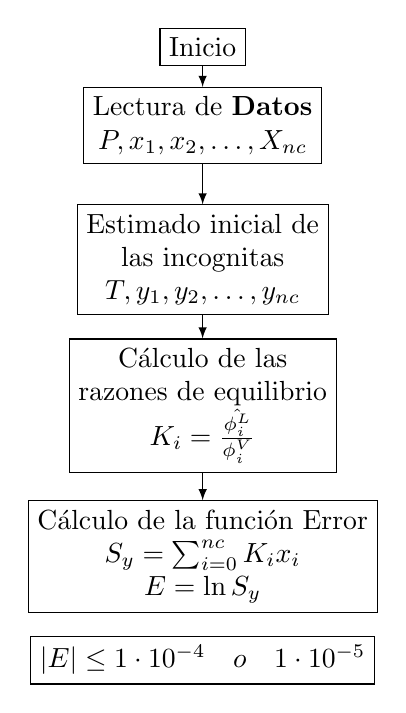
\begin{tikzpicture}[nodes={draw, fill=white,align=center},row sep=0.3cm,column sep=0.5cm] ]

\node(init){Inicio};
\node[below of=init] (lab)  {Lectura de \textbf{Datos} \\$P,x_1, x_2,\ldots, X_{nc}$};
\node[below of=lab,below](estim){Estimado inicial de\\ las incognitas\\$T,y_1,y_2,\ldots,y_{nc}$};
\node[below of=estim,below](relations){Cálculo de las\\ razones de equilibrio\\
$K_i = \frac{ \hat{\phi_i^L} }{ \phi_i^V}$};
\node[below of=relations,below = 0.2cm](error){Cálculo de la función Error\\$ S_y =\sum_{i=0}^{nc} K_i x_i $\\$ E = \ln{S_y} $};

\node[below of=error,below](criteria){$|E| \leq 1\cdot10^{-4}\quad \text{o} \quad  1\cdot 10^{-5}$};

\draw[-latex] (init)--(lab);
\draw[-latex] (lab)--(estim);
\draw[-latex] (estim)--(relations);
\draw[-latex] (relations)--(error);

\end{tikzpicture}

		\subsection{Temperatura de Rocío}\label{subsec:dewtemperature}

	El cálculo de temperatura de rocío para una mezcla se realiza como se indica en la figura \ref{fig:dewtemperature}. Usando un objeto del tipo `HeterogeneousMixture' de la librería \Materia el cálculo se realiza como se muestra en los fragmentos de código \ref{lst:dewtemperature} y \ref{lst:dewtemperatureWithEstimate}.

	Si al método no se le proporciona un estimado inicial, como se muestra en el código \ref{lst:dewtemperature} entonces la clase realiza la estimación de la temperatura como se muestra en la figura \ref{fig:dewtemperatureEstimate}. 

	\begin{lstlisting}[label={lst:dewtemperatureWithEstimate},caption={Cálculo de la temperatura de rocío proporcionando un estimado inicial.}]

		heterogeneousMixture.setZFraction(compound1,molarFraction1);
		//...... asignar la fracción molar para todos los compuestos

		heterogeneousMixture.setPressure(pressure);
		heterogeneousMixture.dewTemperature(temeperatureEstimate,liquidEstimatedFractions);
		double temperature = heterogeneousMixture.getTemperature();
	\end{lstlisting}


	\begin{lstlisting}[label={lst:dewtemperature},caption={Cálculo de la temperatura de rocío.}]

		heterogeneousMixture.setZFraction(compound1,molarFraction1);
		//...... asignar la fracción molar para todos los compuestos

		heterogeneousMixture.setPressure(pressure);
		heterogeneousMixture.dewTemperature();
		double temperature = heterogeneousMixture.getTemperature();
	\end{lstlisting}


		\subsection{Presión de Burbuja}\label{subsec:bubblepressure}

	El cálculo de presión de burbuja para una mezcla se realiza como se indica en la figura \ref{fig:bubblepressure}. Usando un objeto del tipo `HeterogeneousMixture' de la librería \Materia el cálculo se realiza como se muestra en los fragmentos de código \ref{lst:bubblepressure} y \ref{lst:bubblepressureWithEstimate}.

	Si al método no se le proporciona un estimado inicial, como se muestra en el código \ref{lst:bubblepressure} entonces la clase realiza la estimación de la presión de vapor con la ecuación del factor acéntrico \ref{eq:pressureacentricfactor}. 



	\begin{lstlisting}[label={lst:bubblepressureWithEstimate},caption={Cálculo de la presión de burbuja proporcionando un estimado inicial.}]

		heterogeneousMixture.setZFraction(compound1,molarFraction1);
		//...... asignar la fracción molar para todos los compuestos

		heterogeneousMixture.setTemperature(temperature);
		heterogeneousMixture.bubblePressure(
					pressureEstimate,vaporEstimatedFractions);
		double pressure = heterogeneousMixture.getPressure();
	\end{lstlisting}


	\begin{lstlisting}[label={lst:bubblepressure},caption={Cálculo de la presión de burbuja.}]
		heterogeneousMixture.setZFraction(compound1,molarFraction1);
		//...... asignar la fracción molar para todos los compuestos

		heterogeneousMixture.setTemperature(temperature);
		heterogeneousMixture.bubblePressure();
		double pressure = heterogeneousMixture.getPressure();
	\end{lstlisting}

	La figura \ref{fig:bubblepressure3d} muestra los planos obtenidos del líquido saturado y del vapor saturado por medio del cálculo de presión de burbuja para el sistema metanol-agua con la ecuación de PRSV.

\begin{figure}[p]
\centering
	\begin{tikzpicture}
	\begin{axis}[view/v=-15,colorbar left,xlabel={Fracción Molar del metanol},ylabel=\temperature,zlabel=\pressure,colorbar style={ylabel=\temperature,
        yticklabel style={
            text width=2.5em,
            align=right}}]
		\addplot3[surf,point meta=explicit,shader=interp]table[meta=temperature, y=temperature , x=liquidFraction, z=pressure]{plotdata/mixhet/hp.dat};
		\addplot3[surf,point meta=explicit,shader=interp]table[meta=temperature, y=temperature , x=vaporFraction, z=pressure]{plotdata/mixhet/hp.dat};
	\end{axis}
	\end{tikzpicture}


	\begin{tikzpicture}
	\begin{axis}[view/v=-220,xlabel={Fracción Molar del metanol},ylabel=\temperature,zlabel=\pressure]
	\addplot3[surf,point meta=explicit,shader=interp]table[meta=temperature, y=temperature , x=liquidFraction, z=pressure]{plotdata/mixhet/hp.dat};
	\addplot3[surf,point meta=explicit,shader=interp]table[meta=temperature, y=temperature , x=vaporFraction, z=pressure]{plotdata/mixhet/hp.dat};
	\end{axis}
	\end{tikzpicture}


	\begin{tikzpicture}
	\begin{axis}[view/v=-115,xlabel={Fracción Molar del metanol},ylabel=\temperature,zlabel=\pressure]
	\addplot3[surf,point meta=explicit,shader=interp]table[meta=temperature, y=temperature , x=liquidFraction, z=pressure]{plotdata/mixhet/hp.dat};
	\addplot3[surf,point meta=explicit,shader=interp]table[meta=temperature, y=temperature , x=vaporFraction, z=pressure]{plotdata/mixhet/hp.dat};
	\end{axis}
	\end{tikzpicture}
	\caption{Diagramas tridimensionales de presión-composición-temperatura para el sistema metanol-agua. En la figura podemos observar los planos formados por el líquido y el vapor saturado obtenidos con el cálculo de presión de burbuja. Los diagramas son la misma figura vista desde diferentes angulos.}\label{fig:bubblepressure3d}
\end{figure}

		\subsection{Presión de Rocío}\label{subsec:dewpressure}

	El cálculo de presión de rocío para una mezcla se realiza como se indica en la figura \ref{fig:dewpressure}. Usando un objeto del tipo `HeterogeneousMixture' de la librería \Materia el cálculo se realiza como se muestra en los fragmentos de código \ref{lst:dewpressure} y \ref{lst:dewpressureWithEstimate}.

	Si al método no se le proporciona un estimado inicial, como se muestra en el código \ref{lst:dewpressure} entonces la clase realiza la estimación de la presión de vapor con la ecuación del factor acéntrico \ref{eq:pressureacentricfactor}. 

	\begin{lstlisting}[label={lst:dewpressureWithEstimate},caption={Cálculo de la presión de rocío proporcionando un estimado inicial.}]

		heterogeneousMixture.setZFraction(compound1,molarFraction1);
		//...... asignar la fracción molar para todos los compuestos

		heterogeneousMixture.setTemperature(temperature);
		heterogeneousMixture.dewPressure(pressureEstimate);
		double pressure = heterogeneousMixture.getPressure();
	\end{lstlisting}

	\begin{lstlisting}[label={lst:dewpressure},caption={Cálculo de la presión de rocío.}]

		heterogeneousMixture.setZFraction(compound1,molarFraction1);
		//...... asignar la fracción molar para todos los compuestos

		heterogeneousMixture.setTemperature(temperature);
		heterogeneousMixture.dewPressure();
		double pressure = heterogeneousMixture.getPressure();
	\end{lstlisting}

\begin{figure}[!h]
	\begin{tikzpicture}[nodes={draw, fill=white,align=center},row sep=0.3cm,column sep=0.5cm] ]

	\node(init){Inicio};
	\node[below of=init,below] (lab)  {Lectura de \textbf{Datos} \\$T,y_1, y_2,\ldots, y_{nc}$};
	\node[below of=lab,below=0.4](estim){Estimado inicial de\\ las incognitas\\$P,x_1,x_2,\ldots,x_{nc}$};
	\node[below of=estim,below=0.4](relations){Cálculo de las\\ razones de equilibrio\\
	$K_i = \frac{ \hat{\phi}_i^L }{ \hat{ \phi}_i^V}$};
	\node[below of=relations,below = 0.5cm](error){Cálculo de la función Error\\
	$ S_x =\sum_{i=1}^{nc}\frac{y_i}{ K_i} $\\$ E = S_x-1 $};

	\node[below of=error,below=0.4](criteria){$|E| \leq 1\cdot10^{-4}\quad \text{o} \quad  1\cdot 10^{-5}$};
	\node[below of=criteria,below=0.4](tempIncrement){Incrementer la temperatura\\$P^* = P + \Delta P$\\
	$\Delta P = 0.001  \quad \text{o} \quad 0.0001 K$};

	\node[below of=tempIncrement,below=0.4](relationsWithIncrement){Cálculo de las Razones\\ de Equilibrio con $P^*$\\$K_i^* = \frac{ \hat{\phi}_i^L }{\hat{\phi}_i^V}$};

	\node[right of=criteria	,right=2.2cm](end){Fin};


	\node[right of=tempIncrement, right=3cm](errorWithIncrement){Cálculo de la función Error \\ con $P^*$\\
	$ S_x^* =\sum_{i=1}^{nc} \frac{y_i}{K_i^*}  $\\$ E^* = S_x^*-1 $};

	\node[right of=relations, right = 3cm](newValues){Cálculo de las nuevas estimaciones \\ de las \textbf{Incógnitas}\\
	\begin{minipage}{0.2\linewidth}
	\begin{equation*}
	T_{nueva} =P- \frac{E  \left(P^*-P\right)}{E^*-E}
	\end{equation*}
	\begin{equation*}
	 S_x =\sum_{i=1}^{nc}\frac{y_i}{K_i}   \\
	 \end{equation*}
	 \begin{equation*}
	\left(x_i\right)_{nueva} = \frac{y_i}{K_i S_x}
	\end{equation*}
	\end{minipage}
	};


	\draw[-latex] (init)--(lab);
	\draw[-latex] (lab)--(estim);
	\draw[-latex] (estim)--(relations);
	\draw[-latex] (relations)--(error);
	\draw[-latex] (error)--(criteria);
	\draw[-latex] (criteria)--node[fill=none,draw=none,above]{SI}(end);
	\draw[-latex] (criteria)--node[fill=none,draw=none,left]{NO}(tempIncrement);
	\draw[-latex] (tempIncrement)--(relationsWithIncrement);
	\draw[-latex] (relationsWithIncrement)--(errorWithIncrement);
	\draw[-latex] (errorWithIncrement)--(newValues);
	\draw[-latex] (newValues)--(relations);

	\end{tikzpicture}
	\caption{Algoritmo para el cálculo de la presión de rocío.}\label{fig:dewpressure}
\end{figure}
		\subsection{Flash}



\begin{tikzpicture}[nodes={draw, fill=white,align=center},row sep=0.3cm,column sep=0.5cm] ]

\node(init){Inicio};
\node[below of=init] (lab)  {Lectura de \textbf{Datos} \\$T,P,z_1, z_2,\ldots, z_{nc}$};
\node[below of=lab,below](estim){Estimado inicial de\\ las incognitas\\$V/F,x_1,x_2,\ldots,x_{nc}$\\$y_1,y_2 \ldots, y_{nc}$};
\node[below of=estim,below](relations){Cálculo de las\\ razones de equilibrio\\
$K_i = \frac{ \hat{\phi}_i^L }{ \hat{ \phi}_i^V}$};
\node[below of=relations,below = 0.2cm](error){Cálculo de la función Error\\
$ \zeta =\sum_{i=1}^{nc}\left| x_i \hat{\varphi}_i^L - y_i \hat{\varphi}_i^V \right|$};

\node[below of=error,below](criteria){$|\zeta| \leq 1\cdot10^{-4}\quad \text{o} \quad  1\cdot 10^{-5}$};


\node[below of=criteria,below](rachford){Cálculo de $V/F$ con Rachford-Rice:\\ 
\begin{minipage}{0.5\linewidth}
\begin{equation*}
S = \sum_{i=1}^{nc}\frac{z_i\left(K_i - 1\right)}{1+ \frac{V}{F}\left(K_i-1\right)}
\end{equation*}
Encontrar $V/F$ tal que $S = 0$\\
Método de Newton-Raphson\\
\begin{equation*}
\acute{S} = \sum_{i=1}^{nc} \frac{-z_i \left(K_i - 1\right)^2}{\left[1+ \frac{V}{F} \left(K_i-1\right)\right]^2}
\end{equation*}
\begin{equation*}
\left(\frac{V}{F}\right)_{nueva} = \left(\frac{V}{F}\right) - \frac{S}{\acute{S}}
\end{equation*}
\end{minipage}};

\node[right of=criteria	,right=2.2cm](end){Fin};


\node[right of=estim, right = 3cm](newValues){Cálculo de las nuevas estimaciones \\ de las \textbf{Incógnitas}\\
\begin{minipage}{0.3\linewidth}
\begin{equation*}
\acute{x_i} = \frac{z_i}{1 + \frac{V}{F}\left(K_i-1\right)}
\end{equation*}
\begin{equation*}
 S_x =\sum_{i=1}^{nc}\acute{x}_i \qquad x_i = \frac{\acute{x_i}}{S_x}
\end{equation*}
\begin{equation*}
\acute{y_i} = \acute{x_i} K_i = \frac{z_i K_i}{1+\frac{V}{F}\left(K_i - 1\right)}
\end{equation*}
\begin{equation*}
 S_y =\sum_{i=1}^{nc}\acute{y}_i \qquad y_i = \frac{\acute{y_i}}{S_y}
\end{equation*}
\end{minipage}
};


\draw[-latex] (init)--(lab);
\draw[-latex] (lab)--(estim);
\draw[-latex] (estim)--(relations);
\draw[-latex] (relations)--(error);
\draw[-latex] (error)--(criteria);
\draw[-latex] (criteria)--node[fill=none,draw=none,above]{SI}(end);
\draw[-latex] (criteria)--node[fill=none,draw=none,left]{NO}(rachford);

\draw[-latex] (rachford)-|(newValues);
\draw[-latex] (newValues)--(relations);

\end{tikzpicture}

		\subsection{Diagramas}
	



	\chapter{Optimización de parámetros de $\alpha$}
	

\begin{tikzpicture}
\begin{axis}
\addplot[blue,only marks,mark size = 1pt]table[x=temperature, y=exppressure]{plotdata/alphaOptimization/error.dat};
\addplot[green,thick]table[x=temperature,y=calcpressure]{plotdata/alphaOptimization/error.dat};
\addplot[red,thick]table[x=temperature,y=calcpressure]{plotdata/alphaOptimization/minError.dat};
\end{axis}
\end{tikzpicture}

\begin{tabular}{c c c}
\begin{tikzpicture}
	\begin{axis}
		\addplot[red,only marks,mark size = 1pt]table[x=temperature,y=error]{plotdata/alphaOptimization/error.dat};
		\addplot[blue,only marks,mark size = 1pt]table[x=temperature,y=error]{plotdata/alphaOptimization/minError.dat};
	\end{axis}
\end{tikzpicture}
&
\begin{tikzpicture}
	\begin{axis}[width=5cm]
	\addplot[blue,only marks,mark size = 1pt]table[x=temperature,y=error]{plotdata/alphaOptimization/minError.dat};
	\end{axis}
\end{tikzpicture}
\end{tabular}

\begin{tikzpicture}
\begin{axis}
\addplot[orange,only marks,mark size = 1pt]table[x=iteration,y=a]{plotdata/alphaOptimization/trayectory.dat};
\addplot[red,only marks,mark size = 1pt]table[x=iteration,y=b]{plotdata/alphaOptimization/trayectory.dat};
\end{axis}
\begin{axis}
\addplot[blue,only marks,mark size = 1pt]table[x=iteration,y=error]{plotdata/alphaOptimization/trayectory.dat};
\end{axis}
\end{tikzpicture}

\begin{tikzpicture}
\begin{axis}[view/h=80,zmax=614983.3952123278]
\addplot3[surf]table{plotdata/alphaOptimization/params.dat};
\addplot3[red]table[x=a,y=b,z=error]{plotdata/alphaOptimization/trayectory.dat};
\end{axis}
\end{tikzpicture}

\section{Parámetros binarios}
	\chapter{Optimización de parámetros $Binarios$}


\definecolor{amber}{rgb}{1.0, 0.49, 0.0}

\newcommand{\binaryDiagram}[1] {
\begin{tikzpicture}
\begin{axis}
\addplot[amber,only marks,mark size = 1pt]table[x=x1, y=expTemp]{#1};
\addplot[blue,only marks,mark size = 1pt]table[x=yExp, y=expTemp]{#1};
\addplot[green,thick] table[x=x1, y=calcTemp]{#1};
\addplot[red,thick] table[x=yCalc, y=calcTemp]{#1};
\end{axis}
\end{tikzpicture}
 }

\binaryDiagram{plotdata/binaryOptim/error.dat}

\binaryDiagram{plotdata/binaryOptim/errorAfterOptim.dat}
	\chapter{Paquetes termodinámicos}
	\section{Estructura de la librería}
	 \subsection{Materia Homogénea}

			\begin{figure}[!h]
			  
			  \centering
			    \includegraphics[scale=0.7]{Homogenous.png}
			    \caption{A picture of a gull.}
			\end{figure}

		\subsection{Materia Heterogénea}

			\begin{figure}[!h]
			  
			  \centering
			    \includegraphics[scale=0.7]{heterogeneous.png}
			    \caption{ads}
			\end{figure}


	
		\subsection{Mezcla}



	\section{Objetos incluidos}
		\subsection{Ecuaciones de estado cúbicas}
		\subsection{Expresiones de $\alpha$}
		\subsection{Reglas de mezclado}
		\subsection{modelos de actividad}
	\section{¿Cómo extender los paquetes?/ ¿Cómo escribir mi propio paquete?}
		\subsection{Fork Repo desde GitHub}
		\subsection{Agregar classes}
		\subsection{Pull Request}

	\chapter{Aplicación de internet}
	\section{Base de datos}
		\subsection{Usuarios}
		\subsection{Componentes}
		\subsection{Listas de datos experimentales}
			\subsubsection{Compuestos}
			\subsubsection{Mezclas}
	
	\include{advancedOptions_chapter}
	\chapter{Diagramas ternarios}

\newcommand{\alphaOptim}[1] {

\begin{tabular}{c c}

\begin{tikzpicture}
	\begin{axis}
		\addplot[blue,only marks,mark size = 1pt]table[x=Temperature,y=experimentalPressure]{plotdata/ternaryDiagram/#1/afterOptim.dat};
		\addplot[red,thick]table[x=Temperature,y=calculatedPressure]{plotdata/ternaryDiagram/#1/afterOptim.dat};
	\end{axis}
\end{tikzpicture}
&
\begin{tikzpicture}
	\begin{axis}
		\addplot[blue,only marks,mark size = 1pt]table[x=Temperature,y=experimentalPressure]{plotdata/ternaryDiagram/#1/beforeOptim.dat};
		\addplot[red,thick]table[x=Temperature,y=calculatedPressure]{plotdata/ternaryDiagram/#1/beforeOptim.dat};
	\end{axis}
\end{tikzpicture}
\\
\begin{tikzpicture}
	\begin{axis}
		\addplot[blue,only marks,mark size = 1pt]table[x=Temperature,y=error]{plotdata/ternaryDiagram/#1/beforeOptim.dat};
		\addplot[red,only marks,mark size = 1pt]table[x=Temperature,y=error]{plotdata/ternaryDiagram/#1/afterOptim.dat};
	\end{axis}
\end{tikzpicture}
&
\begin{tikzpicture}
	\begin{axis}
		\addplot[only marks,mark size = 1pt]table[x=iteration,y=A]{plotdata/ternaryDiagram/#1/history.dat};
		\addplot[only marks,mark size = 1pt]table[x=iteration,y=B]{plotdata/ternaryDiagram/#1/history.dat};
		\addplot[only marks,mark size = 1pt]table[x=iteration,y=C]{plotdata/ternaryDiagram/#1/history.dat};
	
	\end{axis}
\end{tikzpicture}
\\
\begin{tikzpicture}
	\begin{axis}
		\addplot[red,only marks,mark size = 1pt]table[x=iteration,y=Error]{plotdata/ternaryDiagram/#1/history.dat};
	\end{axis}
\end{tikzpicture}
\end{tabular}
}


\newcommand{\binary}[1]{
\begin{tikzpicture}
	\begin{axis}
		\addplot[blue,only marks,mark size = 1pt]table[x=x1,y=pressure]{plotdata/ternaryDiagram/#1/beforeOptim.dat};
		\addplot[red,only marks,mark size = 1pt]table[x=y1,y=pressure]{plotdata/ternaryDiagram/#1/beforeOptim.dat};
		\addplot[green,thick]table[x=y1calc,y=calcpressure]{plotdata/ternaryDiagram/#1/beforeOptim.dat};
		\addplot[brown,thick]table[x=x1,y=calcpressure]{plotdata/ternaryDiagram/#1/beforeOptim.dat};

		\addplot[purple,thick]table[x=y1calc,y=calcpressure]{plotdata/ternaryDiagram/#1/afterOptim.dat};
		\addplot[black,thick]table[x=x1,y=calcpressure]{plotdata/ternaryDiagram/#1/afterOptim.dat};
	\end{axis}
\end{tikzpicture}

}

\alphaOptim{ethylene}
\alphaOptim{water}
\alphaOptim{ethanol}


binary



\binary{ethylenewater}



\begin{tikzpicture}
\begin{ternaryaxis}[xlabel=Agua,
ylabel=Etileno,
zlabel=Etanol]
\addplot3[only marks,blue] table[x=x1,y=x2,z=x3]{plotdata/ternaryDiagram/graph.dat};
\addplot3[only marks,red] table[x=y1,y=y2,z=y3]{plotdata/ternaryDiagram/graph.dat};
\end{ternaryaxis}
\end{tikzpicture}
	\appendix
	\chapter{Ejemplo de uso con Netbeans}



	\section{Requisitos}

	\begin{enumerate}

		\item Es necesario tener instalado kit de desarrollo Jdk de java que se puede descargar desde la página \url{http://www.oracle.com/technetwork/java/javase/downloads/}.

		\item Es necesario tener instalado el ambiente de desarrollo Netbeans que se puede descargar de la página \url{https://netbeans.org/downloads/}.
	\end{enumerate}

	\section{Instalación manual de la librería Materia}\label{sec:manualInstall}
		Descargar el archivo .jar y agregarlo al folder /lib de la aplicación
		\begin{enumerate}
			\item Desde la página \url{http://hugoredon.github.io/Materia} se puede descargar el archivo jar.

			\item Crear un nuevo proyecto desde Netbeans.

			\begin{center}
			  \includegraphics[scale=0.7]{new-proyect.png}
			\end{center}

			\item Elegir el tipo de aplicación java.application 
			\begin{center}
			  \includegraphics[scale=0.7]{application-type.png} 
			\end{center}
			\item Asignar el nombre del proyecto 
			\begin{center}
			  \includegraphics[scale=0.7]{proyect-name.png} 
			\end{center}
			\item En la pestaña proyectos de netbeans, con click derecho en la carpeta “Libraries” elegir la opción “Agregar jar/Folder “.
			\begin{center}
			  \includegraphics[scale=0.7]{add-jar.png} 
			\end{center}


			 \item Navegar entonces hasta la ruta donde se descargo el archivo jar. 

			\begin{center}
			  \includegraphics[scale=0.7]{select-materia-jar.png} 
			\end{center}

			Se puede ver entonces la librería agregada al proyecto.

			\begin{center}
			  \includegraphics[scale=0.7]{library-added.png} 
			\end{center}
		\end{enumerate}

	\section{Instalación de la librería Materia usando Maven}\label{sec:mavenInstall}

	Para instalar la librería es necesario usar las estructura de archivos de Maven:
	
		    Crear nuevo proyecto :new proyect
		     Elegir la categoría ->Maven ->Java Applicationmaven java app
		    Elegir nombre del proyecto y dar click en finalizar.maven name
		    Podemos ver en la carpeta del proyecto la siguiente estructura
		\begin{verbatim}
		    Maven_Equilibrio
		    |-- pom.xml
		    `-- src
		        -- main
		           `-- java
		               `-- hugo
		                   `-- ejemplos
		                       `-- maven_equilibrio
		\end{verbatim}
		Abrimos el archivo pom.xml y agregamos las siguientes etiquetas


		\begin{lstlisting}[language=XML,morekeywords={repositories,
    repository,id,name,url,groupId,artifactId,dependencies,dependency}]
<repositories>
   <repository>
     <id>snapshots</id>
     <name>snapshotsrepo</name>
     <url>https://oss.sonatype.org/content/repositories/snapshots/</url>
   </repository>
</repositories>
 
<dependencies>
  <dependency>
   <groupId>com.github.hugoredon</groupId>
   <artifactId>materia</artifactId>
   <version>1.2.4-SNAPSHOT</version>
  </dependency>
</dependencies>
\end{lstlisting}


		5- Inmediatamente se ve agregada la dependencia Materia, cuando el proyecto se compile, se descargará el archivo jar automáticamente.

		maven materia added

		6.  Crear una clase java en cualquier paquete dentro de Source packages.maven create java class

		Escribimos dentro de esta clase el mismo código que en la entrada anterior.

	\section{Código}
		\begin{lstlisting}
			
		public class Equilibrio {
		 public static void main(String[] args) {
		 Compound agua = new Compound("agua");
		 agua.setCriticalTemperature(647.3);
		 agua.setCriticalPressure(2.212E7);
		 agua.setAcentricFactor(0.344861);
		 
		 Cubic cubicEquationOfState = EquationOfStateFactory.pengRobinsonBase();
		 Alpha alphaExpression = AlphaFactory.getStryjekAndVeraExpression();
		 
		 HeterogeneousSubstance substance =
		 new HeterogeneousSubstance(cubicEquationOfState, alphaExpression, agua);
		 double pressure = 101325;
		 substance.setPressure(pressure);
		 substance.bubbleTemperature();
		 double temperature = substance.getTemperature();
		 
		 System.out.println("(Presi|ó|n "+pressure+" [Pa])Temperatura de burbuja: " + temperature + "[K]");
		 }
		}

		\end{lstlisting}
		Ejecutamos el código y el resultado es:

		(Presión 101325.0 [Pa])Temperatura de burbuja: 374.5312063949659[K]
	\chapter{¿Cómo extender o modificar la librería dese el código fuente?}\label{chap:github}
	\chapter{Ecuaciones}



\begin{equation}\label{eq:pressure}
P = \frac{R T}{v-b} - \frac{a}{v^2 +u b v + w b^2 }
\end{equation}


\begin{itemize}\itemsep0ex
\item $P$ : presión en $[Pa]$.
\item $v$ : volumen molar en $[\frac{m^3}{kg}]$
\item $a$ : Es una medida de la atracción entre las partículas. $[\frac{m^5}{kg s}]$
\item $b$ : volumen excluido por un mol de partículas.$[\frac{m^3}{kg}]$
\item $u$ y $w$ : Son los parámetros diferentes para cada ecuación de estado, ver tabla \ref{tab:cubics}
\item $R$ : Constante universal de los gases ideales en $\frac{m^3 Pa}{kgmol K}$
\end{itemize}


\begin{equation}\label{eq:a}
	b_i = \Omega_b \frac{R T_{ci}}{p_{ci}} 
\end{equation}

\begin{equation}\label{eq:b}
 a_i = \Omega_a \frac{\left(R T_{ci}\right)^2}{p_{ci}} \alpha_i
\end{equation}


\begin{equation}\label{eq:z}
z= \frac{P V}{R T}
\end{equation}

\begin{equation}\label{eq:volume}
V = \frac{R T}{z P}
\end{equation}

\begin{equation}\label{eq:AB}
A=\frac{ap}{(RT)^2}
\qquad
B=\frac{bp}{RT}
\end{equation}

\begin{equation}
z^3-\left[1-(u-1)B\right]z^2+ \\ \left[A-uB-uB^2 +\\ wB^2\right]z-\left[AB+wB^2+wB^3\right]=0
\end{equation}


\subsubsection{Entalpía del gas ideal}
\begin{equation}\label{eq:idealgasenthalpy}
h^{\neq} = \sum_{i=1}^{nc} x_i \left[ h_i^{ref} + \int_{Tref}^{T} Cp_i^{\neq} \mathrm{d}T \right]
\end{equation}

\section{Entalpía}
\begin{equation}\label{eq:enthalpy}
h = h^{\neq} + \left[ \frac{T(\frac{\partial a}{\partial T}) - a}{b\sqrt{u²-4w} }\right] 
\ln\left[\frac{2v+b\left(u + \sqrt{u²-4w}\right)}{2v+b\left(u - \sqrt{u²-4w}\right)}\right]
+ pv - RT
\end{equation}

\begin{lstlisting}[label=some-code,caption=Some Code]
private  double calculateEnthalpy( double volume){
    double idealGasEnthalpy = calculateIdealGasEnthalpy();
    double a = calculate_a_cubicParameter();
    double b = calculate_b_cubicParameter();
    double L = cubicEquationOfState.calculateL(volume, b);
    double partial_aPartial_temperature = partial_aPartial_temperature( );
    
    return idealGasEnthalpy + ((partial_aPartial_temperature - a)/b) * L  + pressure * volume - Constants.R *temperature;
}
\end{lstlisting}	



\subsection{Entropía}
\begin{equation}
s = s^{\neq} + R\ln\left[\frac{z(v-b)}{v}\right] + \frac{\frac{\partial a}{\partial T}}{b \sqrt{u^2 - 4w}}
\ln\left[\frac{2v+b\left(u + \sqrt{u²-4w}\right)}{2v+b\left(u - \sqrt{u²-4w}\right)}\right]
\end{equation}
\begin{equation}
s^{\neq} = \sum_{i=1}^{nc} x_i\left[s_i^{ref} + \int_{Tref}^T \frac{Cp_i^{\neq}}{T} \mathrm{d}T 
- R\ln \left(\frac{p}{p_{ref}}\right)- R\ln{x_i}
\right]
\end{equation}


\begin{equation}\label{eq:gibbs}
g = h - T * s;
\end{equation}


\begin{multline}\label{eq:fugacity}
\ln\hat{\phi_i} = - \ln\left(\frac{v-b}{v}\right) 
+ (z-1)\left[\frac{1}{b}\frac{\partial bN}{\partial N_i}\right]
+ \frac{a}{RTb\sqrt{u^2-4w}}
\\
\left[\frac{1}{b}\frac{\partial bN}{\partial N_i}
- \frac{1}{aN}\frac{\partial aN²}{\partial N_i}\right]
\ln\left[\frac{2v+b\left(u + \sqrt{u²-4w}\right)}{2v+b\left(u - \sqrt{u²-4w}\right)}\right]
-\ln{z}
\end{multline}

	\bibliographystyle{babplain}
	\bibliography{bib/bibliography}  
\end{document} 